%%%%%%%%%%%%%%%%%%%%%%%%%%%%%%%%%%%%%%%%%%%%%%%%%%%%%%%%%%%%%%%%%%%%%%%%%%%%%%%%%%%%%%%%%%%%%%%%%%%%%%%%%%%%%%%%%%%%%%%%%%%%%%%%%%%%%%%%%%%%%
% Latex Template für Zusammenfassungen
% Robin Frauenfelder - September 2018
%%%%%%%%%%%%%%%%%%%%%%%%%%%%%%%%%%%%%%%%%%%%%%%%%%%%%%%%%%%%%%%%%%%%%%%%%%%%%%%%%%%%%%%%%%%%%%%%%%%%%%%%%%%%%%%%%%%%%%%%%%%%%%%%%%%%%%%%%%%%%



\pagestyle{empty} % Keine Seitennummern

% Verwendete Pakete

	\usepackage[utf8]{inputenc}
	\usepackage[top=0.7cm, bottom=0.9cm, left=0.65 cm, right=0.65 cm, ]{geometry}
	\usepackage{amsmath}
	\usepackage{amsfonts}
	\usepackage{lmodern}
	\usepackage{graphicx}
	\setlength{\parindent}{0pt}
	\usepackage[normalem]{ulem}
	\usepackage[dvipsnames]{xcolor}
	\usepackage{enumitem}
	\usepackage{mathabx}
	\usepackage{enumitem}
	\usepackage{colortbl}
	\usepackage[ngerman]{babel}
	\usepackage{mathtools}
	\usepackage{wallpaper}
	\usepackage{changepage}
	\usepackage{tikz}
	\usepackage{tabularx}
	\usepackage{tcolorbox}
	\usepackage{lipsum}
	\usepackage{multicol}
	\usepackage{letltxmacro}
	\usepackage{tabularx}

% Spalteneinstellungen

	\setlength\columnsep{3mm}
	\setlength{\columnseprule}{0pt}
	
% Neue Befehle

	% Column break
	\newcommand{\colbreak}{%
		\vfill\null
		\columnbreak
	}

	% Bullet-Symbol für Aufzählungen
	\renewcommand\textbullet{\ensuremath{\bullet}}
	
	% Eingekreiste Nummern für Aufzählungen
	\newcommand*\circled[1]{\tikz[baseline=(char.base)]{
            \node[shape=circle,draw,inner sep=1.2pt] (char) {#1};}}
            
    % Horizontale Punkte
    \LetLtxMacro\orgddots\ddots
    \makeatletter
	\DeclareRobustCommand\vdots{%
	  \mathpalette\@vdots{}%
	}
	\newcommand*{\@vdots}[2]{%
	  % #1: math style
	  % #2: unused
	  \sbox0{$#1\cdotp\cdotp\cdotp\m@th$}%
	  \sbox2{$#1.\m@th$}%
	  \vbox{%
	    \dimen@=\wd0 %
	    \advance\dimen@ -3\ht2 %
	    \kern.5\dimen@
	    % remove side bearings
	    \dimen@=\wd2 %
	    \advance\dimen@ -\ht2 %
	    \dimen2=\wd0 %
	    \advance\dimen2 -\dimen@
	    \vbox to \dimen2{%
	      \offinterlineskip
	      \copy2 \vfill\copy2 \vfill\copy2 %
	    }%
	   }%
	}
	\DeclareRobustCommand\ddots{%
		\mathinner{%
		   \mathpalette\@ddots{}%
		   \mkern\thinmuskip
		}%
	}
	
	% Vertikale Punkte
	\DeclareRobustCommand\ddots{%
		  \mathinner{%
		    \mathpalette\@ddots{}%
		    \mkern\thinmuskip
		  }%
		}
		\newcommand*{\@ddots}[2]{%
		  % #1: math style
		  % #2: unused
		  \sbox0{$#1\cdotp\cdotp\cdotp\m@th$}%
		  \sbox2{$#1.\m@th$}%
		  \vbox{%
		    \dimen@=\wd0 %
		    \advance\dimen@ -3\ht2 %
		    \kern.5\dimen@
		    % remove side bearings
		    \dimen@=\wd2 %
		    \advance\dimen@ -\ht2 %
		    \dimen2=\wd0 %
		    \advance\dimen2 -\dimen@
		    \vbox to \dimen2{%
		      \offinterlineskip
		      \hbox{$#1\mathpunct{.}\m@th$}%
		      \vfill
		      \hbox{$#1\mathpunct{\kern\wd2}\mathpunct{.}\m@th$}%
		      \vfill
		      \hbox{$#1\mathpunct{\kern\wd2}\mathpunct{\kern\wd2}\mathpunct{.}\m@th$}%
		    }%
		  }%
		}
	\makeatother
	
	% Schriftart
	\renewcommand{\familydefault}{\sfdefault}
	
	% Dokument-Info Block	
	\newcommand{\DocumentInfo}[3]{
	\begin{tcolorbox}[
			arc=0mm, 
			colback = white!38!black,
			boxrule=0pt,
			toptitle=1mm,
			bottomtitle=1mm,
			right=2mm,
			left=2mm,
			leftright skip = -0.5mm,
			title= \huge \center \textbf{#1} \par \large \vskip1mm #2 \par \vskip1mm \small 	Version: \today,
			fontupper=\color{white},
			after skip = 0 mm,
			top=0.1mm,
			bottom=1mm]
		
		\small #3
	\vskip1mm	
	\end{tcolorbox}
	}
	
	% Überschrift
	\renewcommand{\section}[1]{
	\begin{tcolorbox}[
			arc=0mm,
			colback=white!38!black,
			colframe=white,
			bottomrule = 0 mm,
			toprule = 0 mm,
			leftrule = 0 mm,
			rightrule = 0 mm,
			valign=center,
			left=0.5mm,
			top= 0.7 mm,
			bottom= 0.7 mm,
			fontupper=\color{white},
			before skip = 0mm,
			leftright skip = -0.5mm,
			after skip = 0 mm]

		\textbf{#1}
	\end{tcolorbox}
	}
	
	% Abschnitt	
	\renewcommand{\subsection}[2]{
	\begin{tcolorbox}[
			arc=0mm,
			colback=white!75!black,
			colframe=white,
			bottomrule = 0 mm,
			toprule = 0 mm,
			leftrule = 0 mm,
			rightrule = 0 mm,
			valign=center,
			left=0.5mm,
			top=0.2mm,
			bottom=0.2mm,
			before skip = 0mm,
			leftright skip = -0.5mm,
			after skip = 1.4 mm]
			
		\small \textbf{#1}
	\end{tcolorbox}
	
	\begin{adjustwidth}{0.5mm}{1mm}
		\small
		#2
		\vspace{0.5mm}
	\end{adjustwidth}
	}
	
	% Weisser Balken zwischen Abschnitten
	\newcommand{\WhiteSpace}[0]{
	\begin{tcolorbox}[
			arc=0mm,
			colback=white,
			colframe=white,
			bottomrule = 0 mm,
			toprule = 0 mm,
			leftrule = 0 mm,
			rightrule = 0 mm,
			valign=center,
			left=0.5mm,
			top= -0.2 mm,
			bottom= -0.2 mm,
			fontupper=\color{white},
			before skip = 0mm,
			leftright skip = -0.5mm,
			after skip = 0 mm]
	
	\end{tcolorbox}
	}
	
% Hintergrundbild (graue Spalten)

	\CenterWallPaper{1}{0_Setup/Background.pdf}

% TabularX Zeug (Paket für Tabellen)

	\newcolumntype{Y}{>{\centering\arraybackslash}X}
	\newcolumntype{C}[1]{>{\centering\arraybackslash}p{#1}}
	
% TikZ Zeug (Paket für Vektorgraphiken)

	\usetikzlibrary{decorations.pathreplacing,calc}

	\newcommand{\tikzmark}[2][-3pt]{\tikz[remember picture, overlay, baseline=-0.5ex]\node[#1](#2){};}
	
	\tikzset{brace/.style={decorate, decoration={brace}},
	 brace mirrored/.style={decorate, decoration={brace,mirror}},
	}
	
	\newcounter{brace}
	\setcounter{brace}{0}
	\newcommand{\drawbrace}[3][brace]{%
	 \refstepcounter{brace}
	 \tikz[remember picture, overlay]\draw[#1] (#2.center)--(#3.center)node[pos=0.5, name=brace-\thebrace]{};
	}
	
	\newcommand{\annote}[3][]{%
	 \tikz[remember picture, overlay]\node[#1] at (#2) {#3};
	}

\begin{document}

% Vier Spalten
\begin{multicols*}{4}

% Info über das Dokument
\DocumentInfo
{LinAlg Cheatsheet} %Titel
{Robin Frauenfelder - robinfr@ethz.ch} %Untertitel
{Dieses Cheatsheet wurde im Laufe meiner Übungstunde im MAVT Basisjsahr 18/19 erstellt. Die \LaTeX -Templates findet ihr auf der Amiv-Website.} % Beschreibung
\WhiteSpace

% Dokumentinhalt
\section{1. Lineare Gleichungssysteme}
\WhiteSpace
	\subsection{1.1 Zeilenstufenform}{

Jedes lineare Gleichungssystem kann durch wiederholtes Ausführen folgender drei Rechenoperationen in die sogenannte Zeilenstufenform gebracht werden (Gaussalgorithmus):

\begin{itemize}
\item Zeilen vertauschen
\item Ein Vielfaches einer Zeile zu einer anderen addieren
\item Eine Zeile mit beliebigem Skalar $\neq 0$ multiplizieren
\end{itemize}

\vskip4mm

\renewcommand{\arraystretch}{1.3}
\begin{center}
  \begin{tabular}{C{2mm}  C{2mm}  C{2mm}  C{2mm}  C{2mm}  C{2mm}  C{2mm} | C{2mm}}
    \tikzmark[xshift=-1pt,yshift=4pt]{t}$x_1$ & $x_2$ & $x_3$ & $\dotsm$ & $x_j$ & $\dotsm$ & $x_n$\tikzmark[xshift=0,yshift=4pt]{u} & 1 \\ \hline
    \tikzmark[xshift=-8pt,yshift=1ex]{x}$\oasterisk$ & $\asterisk$ & $\asterisk$ & $\dotsm$ & $\asterisk$ & $\dotsm$ & $\asterisk$ & $b_1$\tikzmark[xshift=8pt,yshift=1ex]{v} \\ \cline{1-2}
    $0$ & $0$ & \multicolumn{1}{|c}{$\oasterisk$} & $\dotsm$ & $\asterisk$ & $\dotsm$ & $\asterisk$ & $b_2$ \\ \cline{3-3}
    $0$ & $0$ & $0$ & $\dotsm$ & $\asterisk$ & $\dotsm$ & $\asterisk$ & $b_1$ \\
    $\vdots$ & $\vdots$ & $\vdots$ &  & $\vdots$ & & $\vdots$ & $\vdots$ \\
    $0$ & $0$ & $0$ & $\dotsm$ & \multicolumn{1}{|c}{$\oasterisk$} & $\dotsm$ & $\asterisk$ & $b_r$\tikzmark[xshift=8pt,yshift=-1ex]{w} \\ \cline{5-7}
    $0$ & $0$ & $0$ & $\dotsm$ & $0$ & $\dotsm$ & $0$ & $b_{r+1}$ \\
    $\vdots$ & $\vdots$ & $\vdots$ &  & $\vdots$ & & $\vdots$ & $\vdots$ \\
    \tikzmark[xshift=-8pt,yshift=-1ex]{y}$0$ & $0$ & $0$ & $\dotsm$ & $0$ & $\dotsm$ & $0$ & $b_m$ \\
  \end{tabular}
\end{center}

\drawbrace[brace mirrored, thick, blue!50!black]{x}{y}
\drawbrace[brace, thick, red!80!black]{v}{w}
\drawbrace[brace, thick, green!50!black]{t}{u}

\annote[above=13mm, left=9pt,  blue!50!black, rotate=90]{brace-1}{m: Anzahl Gleichungen}
\annote[above=5mm, right= 9pt, red!80!black, rotate=-90]{brace-2}{r: Rang}
\annote[above=3pt, green!50!black]{brace-3}{n: Anzahl Unbekannte}

\vspace{-3mm}

\renewcommand{\arraystretch}{2}
\setlength{\tabcolsep}{3pt}
\begin{tabular}{@{} p{2.4cm} p{4.1cm}}
\textbf{Keine Lösung:} & $r < m$ und $b_{i} \neq 0 \hskip3pt \forall i > r$ \\
\textbf{Eindeutige Lösung:} & $r = n = m$ \\
\textbf{Unendlich Lösungen:} & $r < n$ und $b_{i} = 0 \hskip3pt \forall i > r$ \par Anzahl freie Parameter: $n - r$ \\
\textbf{Ax = b für beliebiges b lösbar:} & Voller Rang: $r = m$ \par oder \par $m = n$, und  $Ax = 0$ hat nur die triviale Lösung $x = 0$ \\
\textbf{Ax = b für beliebiges b eindeutig lösbar:} & Voller Rang: $r = m$ und gleich viele Gleichungen wie Unbekannte: $m =n$
\end{tabular}
\vspace{-1mm}
}
\WhiteSpace
	\subsection{1.2 Homogenes Lineares Gleichungssystem}{

\renewcommand{\arraystretch}{1.1}
\begin{center}
  \begin{tabular}{C{3mm}  C{3mm}  C{3mm} C{3.5mm} | C{3mm}}
  $x_1$ &$x_2$ & $\dotsm$ & $x_n$ & 1 \\ \hline
  $a_{11}$ & $a_{12}$ & $\dotsm$ & $a_{1n}$ & \hskip2.2pt 0 \tikzmark[xshift=5pt,yshift=1ex]{vh} \\
  $a_{21}$ & $a_{22}$ & $\dotsm$ & $a_{2n}$ & 0 \\
  $\vdots$ & $\vdots$ &  & $\vdots$ & $\vdots$ \\
  $a_{m1}$ & $a_{m2}$ & $\dotsm$ & $a_{mn}$ & \hskip2.2pt 0 \tikzmark[xshift=5pt,yshift=-1ex]{wh} \\
  \end{tabular}
 \end{center}

\drawbrace[brace, thick, brown!80!black]{vh}{wh}
\annote[above=6.5mm, right= 9pt, brown!80!black, rotate=-90]{brace-4}{\small Nullvektor}

\vspace{-1mm}

\begin{itemize}[leftmargin=0.29cm, itemsep=1pt]

\item Hat immer die triviale Lösung $x = 0$
\item Hat ausschliesslich die triviale Lösung, wenn Rang vollständig ($r = n$, $det(A) \neq 0$)
\item Hat zusätzlich nichttriviale Lösungen, wenn Rang nicht vollständig ($r < n$, $det(A) = 0$)

\end{itemize}

}


	
\section{2. Matrizen}
\WhiteSpace
	\subsection{2.1 Matrixschreibweise}{
	
\vskip1pt
Ein lineares Gleichungssystem kann in Matrixschreibweise dargestellt werden:

\vspace{-1mm}
\begin{center}
\begin{minipage}[t]{0.33\columnwidth}
\renewcommand{\arraystretch}{1.1}
  \begin{tabular}{C{2mm}  C{2.5mm} | C{2mm}}
  $x_1$ & $x_2$ & 1 \\ \hline
  $a_{11}$ & $a_{12}$ & $b_1$  \\
  $a_{21}$ & $a_{22}$ &  $b_2$  \\
  $a_{31}$ & $a_{32}$ &  $b_3$  \\
  \end{tabular}
\end{minipage}
\begin{minipage}[t]{0.12 \columnwidth}
$\Longleftrightarrow$
\end{minipage}
\begin{minipage}[t]{0.5 \columnwidth}
$\begin{pmatrix}
  a_{11} & a_{12} \\
  a_{21} & a_{22} \\
  a_{31} & a_{32} \\
\end{pmatrix}$
$\cdot$
$\begin{pmatrix}
x_1 \\
x_2
\end{pmatrix}$
$=$
$\begin{pmatrix}
b_1 \\
b_2 \\
b_3
\end{pmatrix}$
\end{minipage}
\end{center}
}
\WhiteSpace
	\subsection{2.2 Matrixmultiplikation}{
\vskip1pt
Matrizen können auf folgende Weise miteinander multipliziert werden:

\begin{center}
\fbox{
$A \cdot B = C \hspace{5pt} \Rightarrow \hspace{5pt} c_{ik} = \sum_{j=1}^n a_{ij} \cdot b_{jk}$
}
\end{center}

\vspace{-2mm}

\begin{center}
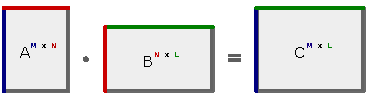
\includegraphics[width = 0.95 \columnwidth]{2_Matrizen/Matrixmultiplikation.pdf}
\end{center}



\textbf{Assoziativ- \& Distributivgesetz:}

\vspace{-6mm}
\begin{center}
\parskip3pt
\begin{align}
(A\cdot B) \cdot C &= A \cdot (B \cdot C) \nonumber \\
(A + B) \cdot C &= A \cdot C + B \cdot C \nonumber \\
A \cdot (C + D) &= A \cdot C + A \cdot D \nonumber
 \end{align}
\end{center}
\textbf{Achtung!} Kommutativgesetz gilt nicht! i.A. $A\cdot B \neq B \cdot A$
}
\WhiteSpace
	\subsection{2.3 Identitätsmatrix}{

\vskip1pt
Die Identitäts- oder Einheitsmatrix ist eine quadratische Matrix, deren Hauptdiagonalenelemente 1 und deren Ausserdiagonalelemente 0 sind.

\begin{center}
$I_n =$
$\begin{pmatrix}
1 & 0 & \dotsm & 0 \\
0 & 1 & \dotsm & 0 \\
\vdots & \vdots & & \vdots \\
0 & 0 & \dotsm & 1
\end{pmatrix}$
$\in \mathbb{R}^{n \times n}$
\end{center}

\textbf{Rechenregel:}
$A^{m \times n} \cdot I_n = I_m \cdot A^{m \times n} = A^{m \times n}$

}
\WhiteSpace
	\subsection{2.4 Diagonal- und Dreiecksmatrizen}{

\vskip1pt

Eine \textbf{Diagonalmatrix} ist eine quadratische Matrix, deren Elemente ausserhalb der Hauptdiagonalen 0 sind.

\begin{center}

$ D = diag(d_1, d_2, d_3) = \begin{pmatrix} d_1 & 0 & 0 \\ 0 & d_2 & 0 \\ 0 & 0 & d_3 \end{pmatrix}$

\end{center}

Eine \textbf{Dreiecksmatrix} ist eine quadratische Matrix, deren Elemente entweder oberhalb oder unterhalb der Hauptdiagonalen Null sind. Man unterscheidet zwischen einer \textbf{Rechtsdreiecksmatrix} und einer \textbf{Linksdreiecksmatrix.}

\begin{center}

$ R = \begin{pmatrix} r_{11} & r_{12} & r_{13} \\ 0 & r_{22} & r_{23} \\ 0 & 0 & r_{33} \end{pmatrix}$
\hskip10pt
$ L = \begin{pmatrix} l_{11} & 0 & 0 \\ l_{21} & l_{22} & 0 \\ l_{31} & l_{32} & l_{33} \end{pmatrix}$

\end{center}

\textbf{Für Diagonal- und Dreiecksmatrizen gilt:} \par
\begin{itemize}[leftmargin=0.29cm, itemsep=0.8pt]
\item $det(A) = a_{11} \cdot a_{22} \cdot a_{33}   \dotsm a_{nn}$
\item $eig(A) = \{a_{11}, a_{22}, \cdots ,  a_{nn}\}$
\end{itemize}

}
	\subsection{2.5 Transponierte}{
\vskip1pt
Die Transponierte einer Matrix erhält man, indem man sie an ihrer Diagonalen \glqq spiegelt\grqq.

\vspace{0.5mm}

\begin{center}

\textbf{Bsp:} 
$\begin{pmatrix}
a & b \\
c & d \\
e & f \\
\end{pmatrix}^T
=
\begin{pmatrix}
a & c & e \\
b & d & f \\
\end{pmatrix}$

\end{center}

\textbf{Rechenregeln:} \par
\vspace{-1.5mm}
\begin{minipage}[t]{0.49 \columnwidth}
\begin{align}
(A + B)^T &= A^T + B^T \nonumber \\
(A \cdot B)^T &= B^T \cdot A^T \nonumber \\
(c \cdot A)^T &= c \cdot A^T \nonumber \\
(A^T)^T &= A \nonumber
\end{align}
\end{minipage}
\begin{minipage}[t]{0.49 \columnwidth}
\begin{align}
(A^T)^{-1} &= (A^{-1})^T \nonumber \\
rang(A^T) &= rang(A) \nonumber \\
det(A^T) &= det(A) \nonumber \\
eig(A^T) &= eig(A) \nonumber
\end{align}
\end{minipage}


}
\WhiteSpace
	\subsection{2.6 Inverse}{

Die Inverse $A^{-1}$ von $A$ macht eine Multiplikation mit $A$ rückgängig. Multipliziert man $A$ mit $A^{-1}$, erhält man die Identitätsmatrix.

\vspace{0pt}

\begin{center}
\fbox{\parbox[c][0.7cm][t]{0.55\columnwidth }{\centering $A\cdot v = w \Leftrightarrow A^{-1}\cdot w = v$ 
\\\addvspace{3pt}
$A^{-1} \cdot A = A \cdot A^{-1} = I$}}
\end{center}

\textbf{Eigenschaften:}

 \vspace{-3pt}

\begin{itemize}[leftmargin=0.29cm, itemsep=0pt]
\item Nur quadratische Matrizen können invertierbar sein.
\item Eine invertierbare Matrix nennt man \textbf{regulär}, eine nicht invertierbare \textbf{singulär}.
\item Die Inverse ist eindeutig.
\item $A$ ist invertierbar $\Longleftrightarrow$ $A$ hat vollen Rang
\item $A$ ist invertierbar $\Longleftrightarrow$ $A^T$ ist invertierbar
\item $A$ ist symmetrisch $\Longleftrightarrow$ $A^{-1}$ ist symmetrisch
\item $A$ ist eine Dreiecksmatrix $\Longleftrightarrow$ $A^{-1}$ ist eine Dreiecksmatrix
\item $A$ ist invertierbar $\Longleftrightarrow$ $det(A) \neq 0$
\item $A$ ist invertierbar $\Longleftrightarrow$ kein Eigenwert $\lambda = 0$
\item $A$ und $B$ sind invertierbar $\Longrightarrow$ $AB$ ist invertierbar
\end{itemize}

\vskip0mm

\textbf{Gauss-Jordan Algorithmus:}\par
\vspace{1mm}
Methode zur Bestimmung der Inversen. Man schreibt die Matrix und die Identität nebeneinander auf und führt den Gaussalgorithmus gleich auf beiden Seiten aus, sodass am Ende auf der linken Seite die Identitätsmatrix steht. \par
\textbf{Tipp:} Erzeuge zuerst durch \glqq nach unten gaussen\grqq \hskip2pt links eine Rechtsdreiecksmatrix, dann durch \glqq nach oben gaussen\grqq  \hskip2pt eine Diagonalmatrix, und am Ende durch Zeilenmultiplikation die Identitätsmatrix.

\vskip1.5mm

\scalebox{0.97}{
\hspace{-2mm}
\begin{minipage}[c]{0.44 \columnwidth}
$\begin{pmatrix}
1 & 2 & 0 & \multicolumn{1}{|c}{1} & 0 & 0 \\
2 & 3 & 0 & \multicolumn{1}{|c}{0} & 1 & 0 \\
\tikzmark[xshift=0,yshift=-6pt]{i_1} 3 & 4 & 1 \tikzmark[xshift=0,yshift=-6pt]{i_2} & \multicolumn{1}{|c}{0} & 0 & 1 \\
\end{pmatrix}$
\end{minipage}
\begin{minipage}[t]{0.041 \columnwidth}
\begin{center}
$\Rightarrow$
\end{center}
\end{minipage}
\begin{minipage}[c]{0.38 \columnwidth}
$\begin{pmatrix}
1 & 0 & 0 & \multicolumn{1}{|c}{-3} & 2 & 0 \\
0 & 1 & 0 & \multicolumn{1}{|c}{2} & -1 & 0 \\
0 & 0 & 1 & \multicolumn{1}{|c}{\tikzmark[xshift=0,yshift=-6pt]{i_3} 1} & -2 & 1 \tikzmark[xshift=0,yshift=-6pt]{i_4} \\
\end{pmatrix}$
\end{minipage}

\drawbrace[brace mirrored, thick, blue!50!black]{i_1}{i_2}
\drawbrace[brace mirrored, thick, red!80!black]{i_3}{i_4}
\annote[below=3pt, blue!50!black]{brace-5}{\small $A$}
\annote[below=3pt, red!80!black]{brace-6}{\small $A^{-1}$}
}

\vskip5mm

\textbf{Adjunktenformel für 2x2-Matrizen:}
\vspace{2pt}

\begin{center}
$\begin{pmatrix}
a & b \\
c & d 
\end{pmatrix}^{-1}
=
\dfrac{1}{ad - bc} \cdot
\begin{pmatrix}
d & -b \\
-c & a 
\end{pmatrix}$
\end{center}

\vskip0mm

\textbf{Rechenregeln:} \par
\vspace{-2.5mm}
\begin{minipage}[t]{0.49 \columnwidth}
\begin{align}
I^{-1} &= I\nonumber \\
(A^{-1})^{-1} &= A \nonumber \\
(A^k)^{-1} &= (A^{-1})^k \nonumber \\
(c\cdot A)^{-1} &= c^{-1} \cdot A^{-1} \nonumber \\
(A\cdot B)^{-1} &= B^{-1} \cdot A^{-1} \nonumber
\end{align}
\end{minipage}
\begin{minipage}[t]{0.49 \columnwidth}
\begin{align}
(A^T)^{-1} &= (A^{-1})^T \nonumber \\
rang(A^{-1}) &= rang(A) \nonumber \\
det(A^{-1}) &= det(A)^{-1} \nonumber \\
eig(A^{-1} &= eig(A)^{-1} \nonumber 
\end{align}
\end{minipage}

}
	\subsection{2.7 Orthogonale Matrizen}{


Eine quadratische Matrix ist orthogonal, wenn sie aus \textbf{zueinander orthogonalen Spaltenvektoren der Länge 1} besteht. Dies ist der Fall, wenn eine Matrix mit der Transponierten multipliziert die Identität ergibt.

%\vspace{-5pt}

\begin{center}
\fbox{$Q^T \cdot Q = I$}
\end{center}

Multipliziert man einen Vektor mit einer orthogonalen Matrix, kann sich seine Orientierung ändern, jedoch nicht seine Länge. Abbildungen sind deshalb kongruent.

\vskip5pt

\textbf{Eigenschaften:}

\vspace{-3pt}

\begin{itemize}[leftmargin=0.29cm, itemsep=0.5pt]
\item $Q$ orthogonal $\Leftrightarrow$ Spalten/Zeilen von $Q$ sind zueinander orthogonale Vektoren der Länge 1.
\item Nur quadratische Matrizen können orthogonal sein.
\item $A$ und $B$ orthogonal $\Rightarrow$ $A \cdot B$ orthogonal
\item $Q$ orthogonal $\Leftrightarrow$ $Q^{-1}$ orthogonal
\item $\|Qx\|_2 = \|x\|_2$, $|det(Q)| = 1$, $|eig(Q)| = 1$
\item $Q^{-1} = Q^T$
\end{itemize}
\vspace{-5pt}

%\textbf{Drehungs- und Spiegelungsmatrizen:}
%
%\vskip1pt
%
%Drehung um Ursprung im $\mathbb{R}^2$: \par \vspace{-1mm} \begin{center}$R(\alpha) = \begin{pmatrix} cos(\alpha) & - sin(\alpha) \\ sin(\alpha) & cos(\alpha) \end{pmatrix}$\end{center} \par
%Drehung um x-Achse im $\mathbb{R}^3$: \par \vspace{-1mm} \begin{center}
%$R_x(\alpha) = \begin{pmatrix} 1 & 0 & 0 \\ 0 & cos(\alpha) & -sin(\alpha) \\ 0 & sin(\alpha) & cos(\alpha)  \end{pmatrix}$ \end{center}
%Drehung um y-Achse im $\mathbb{R}^3$: \par \vspace{-1mm} \begin{center}
%$R_y(\alpha) = \begin{pmatrix} cos(\alpha) & 0 & sin(\alpha) \\ 0 & 1 & 0 \\ -sin(\alpha) & 0 & cos(\alpha)  \end{pmatrix}$ \end{center}
%Drehung um z-Achse im $\mathbb{R}^3$: \par \vspace{-1mm} \begin{center}
%$R_z(\alpha) = \begin{pmatrix} cos(\alpha) & -sin(\alpha) & 0 \\ sin(\alpha) & cos(\alpha) & 0 \\ 0 & 0 & 1  \end{pmatrix}$ \end{center}
%
%
}
\WhiteSpace
	\subsection{2.8 LR-Zerlegung}{

\vspace{2pt}
\begin{center}
\fbox{$A = L \cdot R$}
\end{center}
\vspace{6pt}

Mit der LR-Zerlegung kann man eine quadratische Matrix $A$ in das Produkt einer Linksdreiecksmatrix $L$ sowie einer Rechtsdreiecksmatrix $R$ zerlegen. Dies ermöglicht ein effizienteres Lösen von $Ax = b_i$ mit vielen verschiedenen $b_i$.

\vspace{3pt}
\begin{center} \scalebox{0.9}{Bsp: Löse $Ax = b$ durch LR-Zerlegung von $A = \begin{pmatrix} 2 & 5 \\ 4 & 12 \end{pmatrix}$} \end{center}
\vspace{0pt}

\textbf{Vorgehen:}
\vskip2pt

\begin{enumerate}[label=\protect\circled{\arabic*}]
\item Bringe A durch Zeilensubtraktion in Dreiecksform. Bei erzeugten Nullstellen speichert man, das Wievielfache einer anderen Zeile von dieser Zeile subtrahiert wurde. 
\vskip6pt Bsp: \scalebox{0.8}{\hskip8pt$\begin{pmatrix} 2 & 5 \\ 4 & 12 \end{pmatrix}  \hskip3pt \Longrightarrow \hskip3pt$} \scalebox{0.7}{$\begin{pmatrix} 2 & 5 \\ \boxed{2} & 2 \end{pmatrix}$} \par
\scalebox{0.7}{\hskip35pt $\boxed{2}$: Von dieser Zeile wurde das 2-fache einer anderen subtrahiert.}

\item Bestimme $L$ und $R$. $L$ besteht aus den markierten Einträgen und 1 auf der Diagonale, $R$ aus den nichtmarkierten Einträgen.
\vskip6pt Bsp: \scalebox{0.7}{\hskip8pt$\begin{pmatrix} \textcolor{Maroon}{2} & \textcolor{Maroon}{5} \\ \textcolor{OliveGreen}{\boxed{2}} & \textcolor{Maroon}{2} \end{pmatrix}$} \scalebox{0.8}{$\Longrightarrow \hskip2pt \textcolor{OliveGreen}{L = \begin{pmatrix} 1 & 0 \\ 2 & 1 \end{pmatrix}}, \hskip3pt \textcolor{Maroon}{R = \begin{pmatrix} 2 & 5 \\ 0 & 2 \end{pmatrix}}$}\par

\item Löse $Ly = b$ (einfach, da $L$ eine Dreiecksmatrix).
\item Löse $Rx = y$ (einfach, da $R$ eine Dreiecksmatrix).
\end{enumerate}
\vskip5pt

\textbf{LRP-Zerlegung mit Permutationsmatrix P}

\vspace{5pt}
\begin{center}
\fbox{$P \cdot A = L \cdot R$}
\end{center}
\vspace{2pt}

Manchmal ist es notwendig, dass man bei \circled{1} zusätzlich Zeilen vertauschen kann. Dies wird durch eine Permutationsmatrix $P$ möglich. \par
Hierzu schreibe man zu Beginn die Identitätsmatrix neben $A$, und macht mit dieser alle Zeilenvertauschungen mit:

\vspace{3pt}
\begin{center} \scalebox{0.9}{Bsp: \hskip6pt
$\begin{pmatrix}
1 & 0  & \multicolumn{0}{|c}{1} & 2 \\
0 & 1  & \multicolumn{1}{|c}{3} & 4 \\
\end{pmatrix}
\Longrightarrow
\begin{pmatrix}
0 & 1  & \multicolumn{0}{|c}{3} & 4 \\
1 & 0  & \multicolumn{1}{|c}{1} & 2 \\
\end{pmatrix}
$} \end{center}
\vspace{3pt}

Auf der linken Seite steht am Ende die Permutationsmatrix $P$. $L$ und $R$ werden auf die gleiche Weise wie üblich bestimmt. Bei \circled{3} löse man nun $Ly = Pb$, bei \circled{4} weiterhin $Rx = y$. \par
}
\newpage
	\subsection{2.9 Symmetrische Matrizen}{
\vskip1pt

\textbf{Symmetrische Matrix}\vskip2pt
Eine symmetrische Matrix ist eine quadratische Matrix, deren Einträge spiegelsymmetrisch bezüglich der Hauptdiagonalen sind. \par
Dies ist der Fall, wenn sie gleich ihrer Transponierten ist:


\begin{center}
\fbox{$S = S^T$}
\end{center}


\textbf{Eigenschaften:}
\vspace{-3pt}

\begin{itemize}[leftmargin=0.29cm, itemsep=0.5pt]
\item $A^T A$ und $A A^T$ sind immer symmetrisch.
\item Die Eigenwerte von $S$ sind alle reell.
\item Ist $x$ ein Eigenvektor von $S$ zum Eigenwert $\lambda$, so sind auch $konj(x)$, $Re(x)$, $Im(x)$ Eigenvektoren zum selben Eigenwert $\lambda$
\item Die Eigenvektoren zu unterschiedlichen Eigenwerten sind orthogonal zueinander.
\item $S$ ist halbeinfach, also diagonalisierbar.
\item $S$ besitzt eine orthonormale Eigenbasis.
\item Transformationsmatrix $T$ in Eigenbasis kann orthogonal gewählt werden.
\item $S = (s_{ij}) \in \mathbb{R}^{n \times n}$ mit $s_{ij} = s_{ji}$
\end{itemize}\vskip4pt

\textbf{Schiefsymmetrische Matrix}\vskip2pt
Eine schiefsymmetrische Matrix ist eine quadratische Matrix, welche gleich dem Negativen ihrer Transponierten ist:


\begin{center}
\fbox{$-S = S^T$}
\end{center}


\textbf{Eigenschaften:}
\vspace{-3pt}

\begin{itemize}[leftmargin=0.29cm, itemsep=0.5pt]
\item Die Eigenwert von $S$ sind alle imaginär oder gleich 0
\item Alle Diagonaleinträge sind notwendigerweise gleich 0
\item $det(S) = det(S^T) = det(-S) = (-1)^n det(S)$
\item $S = (s_{ij}) \in \mathbb{R}^{n \times n}$ mit $s_{ij} = -s_{ji}$
\end{itemize}
\vspace{-2mm}

}
\WhiteSpace
	
\section{3. Determinante}
\WhiteSpace
	\subsection{3.1 Definition Determinante}{
\vskip1pt

Die Determinante ist eine Zahl, die einer quadratischen Matrix zugeordnet wird und aus ihren Einträgen berechnet werden kann. Die folgenden Spalten/zeileneigenschaften sind Teil ihrer Definition.

\vskip3pt

\textbf{Zeileneigenschaften:}
\vskip2pt

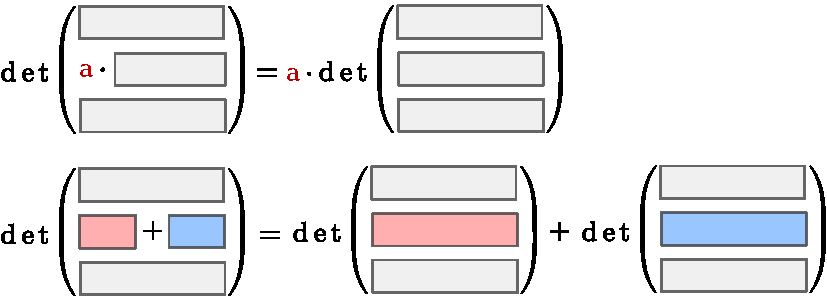
\includegraphics[width = 0.95 \columnwidth]{3_Determinante/Det_Zeilen.pdf}

\begin{itemize}[leftmargin=0.29cm, itemsep=0.5pt]
\item Vertauscht man zwei Zeilen von A, so ändert sich das Vorzeichen der Determinante. 
\item Addiert man ein Vielfaches einer Zeile zu einer anderen, so ändert sich die Determinante nicht.
\end{itemize}

\vskip2pt

\textbf{Spalteneigenschaften:}
\vskip2pt

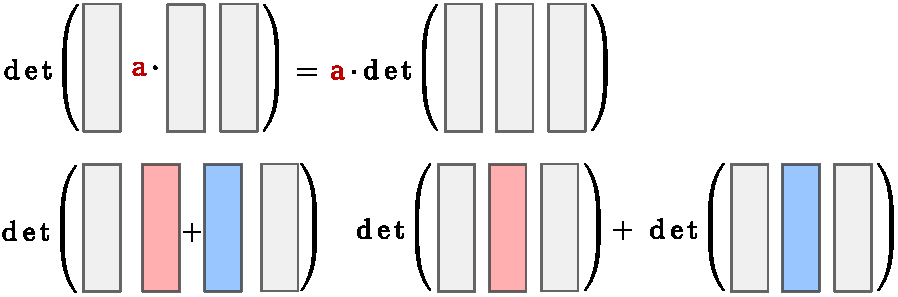
\includegraphics[width = 0.95 \columnwidth]{3_Determinante/Det_Spalten.pdf}

\begin{itemize}[leftmargin=0.29cm, itemsep=0.5pt]
\item Vertauscht man zwei Spalten von A, so ändert sich das Vorzeichen der Determinante. 
\item Addiert man ein Vielfaches einer Spalte zu einer anderen, so ändert sich die Determinante nicht.
\end{itemize}


\vskip2pt

\textbf{Folgerungen aus Zeilen/Spalteneigenschaften:}
\vskip2pt
\begin{itemize}[leftmargin=0.29cm, itemsep=0.5pt]
\item Hat A zwei gleiche Zeilen/Spalten, so gilt $det(A) = 0$.
\item Hat A eine Nullzeile/spalte, so gilt $det(A) = 0$
\item $det(\alpha \cdot A^{n \times n}) = \alpha^n \cdot det(A)$
\end{itemize}

}
\WhiteSpace
	\subsection{3.2 Rechenregeln Determinante}{
\vskip1pt
Neben den Zeilen/Spalteneigenschaften von 3.1 gelten folgende Rechenregeln: \par
\vspace{-3mm}

\hskip5pt
\begin{minipage}[t]{0.7 \columnwidth}
\begin{align}
det(A B) &= det(A) \cdot det(B)\nonumber \\
det(A^T) &= det(A) \nonumber \\
det(diag(d_{1}, d_{2}, \dotsm, d_n)) &= d_1 \cdot d_2 \dotsm d_n \nonumber \\
det(Dreiecksmatrix) &= d_1 \cdot d_2 \dotsm d_n \nonumber \\
det(A^{-1}) &= 1/det(A) \nonumber
\end{align}
\end{minipage}

}
\WhiteSpace
	\subsection{3.3 Berechnungsmethoden Determinante}{
\vskip1pt
Es gibt verschiedene Methoden, die Determinante zu bestimmen. Je nach Matrix eignen sich unterschiedliche Rechnungswege oder Kombinationen davon.

\vskip8pt

\textbf{Fertige Formeln} \par
\vskip1pt
Eignen sich nur bei kleinen Matrizen. Meistens für 3x3-Matrix bereits zu kompliziert.
\vskip6pt
\setlength\parindent{4pt}
\textbf{1x1:} $|a| = a$ \par
\vskip4pt
\textbf{2x2:} $\begin{vmatrix} a & b \\ c & d \end{vmatrix} = a d - c b$ \par
\vskip4pt
\textbf{3x3:} $\begin{vmatrix} a & b & c \\ d & e & f \\ g & h & i \end{vmatrix} = aei + bfg +cdh - gec -hfa -idb $
\setlength\parindent{0pt}
\vskip10pt

\textbf{Laplace'scher Entwicklungssatz:} \par
\vskip1pt
Bei den meisten Matrizen ineffizient. Kann jedoch bei Matrix mit vielen Nullen in einer Zeile oder Spalte geschickt angewendet werden.

\begin{enumerate}[label=\protect\circled{\arabic*}]
\item Zeile oder Spalte auswählen (dort wo viele Nullen).
\item Jedem Element dieser Zeile/Spalte ein Vorzeichen zuordnen (Schachbrett).
\item Für jedes Element die zugehörige Zeile und Spalte streichen und Unterdeterminante bestimmen.
\item Jede Unterdeterminante mit zugehörigem Element und Vorzeichen multiplizieren und addieren.
\end{enumerate}
\hskip3pt \textbf{Bsp:} Entwicklung nach erster Spalte: \par
\vskip3pt
\hskip3pt$\begin{vmatrix} \textbf{\textcolor{NavyBlue}{1}} & 2 & 1 \\ \textbf{\textcolor{NavyBlue}{3}} & 8 & 5 \\ \textbf{\textcolor{NavyBlue}{0}} & 3 & 2 \end{vmatrix} = \textcolor{Maroon}{+} \hskip1pt \textbf{\textcolor{NavyBlue}{1}} \cdot \begin{vmatrix} 8 & 5 \\ 3 & 2 \end{vmatrix} \textcolor{Maroon}{-} \hskip1pt \textbf{\textcolor{NavyBlue}{3}} \cdot \begin{vmatrix} 2 & 1 \\ 3 & 2 \end{vmatrix} \textcolor{Maroon}{+} \hskip1pt \textbf{\textcolor{NavyBlue}{0}}$ \hskip6pt \scalebox{.7}{\color{Maroon}$\begin{pmatrix} + & - & + \\ - & + & - \\ + & - & + \end{pmatrix}$}
\vskip12pt

\textbf{Anwenden von Zeilen/Spalteneigenschaften} \par
\vskip1pt
Durch vertauschen von Spalten/Zeilen (Vorzeichenänderung) oder Zeilen/Spaltenaddition (Determinante bleibt gleich) lässt sich die Matrix oft in eine einfachere Form bringen.
\vskip10pt

\textbf{Blocksatz} \par
Oft in Kombination mit \glqq Anwenden von Zeilen/Spalteneigen- schaften\grqq \hskip1pt nützlich. \par
\vspace{0pt}
\begin{center}
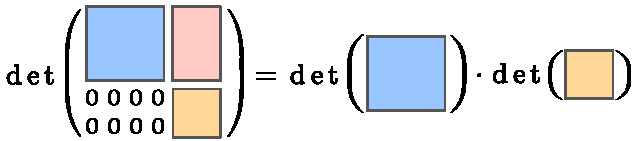
\includegraphics[width = 0.8 \columnwidth]{3_Determinante/Blocksatz.pdf}
\end{center}

\textbf{LR-Zerlegung} \par
\vskip1pt
Nur sinnvoll, wenn LR-Zerlegung bereits vorliegt. \par
\vskip4pt
$det(A) = (-1)^{\# Zeilenvertauschungen} \cdot r_{11} \cdot r_{22} \dotsm r_{nn}$

}
\WhiteSpace
	\subsection{3.4 Wichtige Zusammenhänge}{
\vspace{-1pt}

Folgende Aussagen sind für $A^{n \times n}$ äquivalent:

\vspace{-5pt}
\begin{itemize}[leftmargin=0.29cm, itemsep=0pt]
\item $rang(A) = n$
\item Das LGS $Ax = b$ ist für beliebiges b lösbar.
\item Das LGS $Ax = b$ besitzt genau eine Lösung.
\item Das homogene LGS $Ax = 0$ besitzt nur die triviale Lösung.
\item Die Zeilen/Spalten von A sind linear unabhängig.
\item $A$ ist invertierbar.
\item $det(A) \neq 0$
\item Die Spalten von A bilden eine Basis in $\mathbb{R}^n$.
\item Der Kern von $A$ besteht nur aus dem Nullvektor.
\item Kein Eigenwert von $A$ ist 0.
\item A ist regulär.
\item A ist nicht singulär.
\end{itemize}
\vspace{-2.5mm}

}
\WhiteSpace
	
\section{4. Vektorräume}
\WhiteSpace
	\subsection{4.1 Definition Vektorraum}{
\vskip1pt
Sei V eine Menge von Objekten. V heisst Vektorraum, wenn eine \textbf{innere Operation} (Kombination von zwei Objekten) und eine \textbf{äussere Operation} (Kombination eines Objekts mit einem Skalar) definiert sind, und folgende Axiome gelten:

\vskip3pt
\hskip6pt
\begin{minipage}[c]{0.35 \columnwidth}
\textbf{Innere Operation:}
\vskip1pt
$\bigoplus$: \hskip2pt $V \times V \rightarrow V$ \par
\hskip15pt $(a, b) \mapsto a \bigoplus b$
\end{minipage}
\hskip30pt
\begin{minipage}[c]{0.35 \columnwidth}
\textbf{Äussere Operation:}
\vskip1pt
$\bigodot$: \hskip2pt $\mathbb{K} \times V \rightarrow V$ \par
\hskip15pt $(\alpha, a) \mapsto \alpha \bigodot a$
\end{minipage}

\vskip3pt
\hskip6pt
\textbf{Axiome:} \vskip2pt \par
\hskip6pt
\begin{minipage}[t]{0.36 \columnwidth}
\parskip8pt
(A1) $\forall u, v \in V:$ \par
(A2) $\forall u, v, w \in V:$ \par
(A3) $\exists 0 \in V,$ \par \vspace{-4pt}
\hskip17pt $\forall u \in V:$ \par
(A4) $\forall u \in V,$ \par \vspace{-4pt}
\hskip17pt $\exists -u \in V:$
\end{minipage}
\begin{minipage}[t]{0.6 \columnwidth}
\parskip8pt
$u \bigoplus v = v \bigoplus u$ \par
$(u \bigoplus v) \bigoplus w = u \bigoplus (v \bigoplus w)$ \par
$u \bigoplus 0 = u$ \par \vskip12pt
$u \bigoplus (-u) = 0$
\end{minipage}

\vskip12pt
\hskip6pt
\begin{minipage}[t]{0.36 \columnwidth}
\parskip8pt
(M1) $\forall \alpha, \beta \in \mathbb{R},$ \par \vspace{-4pt}
\hskip17pt $\forall u \in V:$ \par
(M2) $\forall \alpha, \beta \in \mathbb{R},$ \par \vspace{-4pt}
\hskip17pt $\forall u, v \in V:$ \par
(M3) $\forall u \in V:$
\end{minipage}
\begin{minipage}[t]{0.6 \columnwidth}
\parskip8pt
$(\alpha \cdot \beta) \bigodot u = \alpha \bigodot (\beta \bigodot u)$ \par \vskip12pt
$(\alpha + \beta) \bigodot u = (\alpha \bigodot u) \bigoplus (\beta \bigodot u)$ \par \vskip-4pt
$\alpha \bigodot (u \bigoplus v) = (\alpha \bigodot u) \bigoplus (\alpha \bigodot v)$
\vskip0pt
$1 \bigodot u = u$

\end{minipage}

}
\WhiteSpace
	\subsection{4.2 Definition Unterraum}{
\vskip1pt
Eine nichtleere Teilmenge eines Vektorraums V heisst Unterraum von V, falls:
\vskip6pt
\begin{enumerate}[label=\protect\circled{\arabic*}]
\item \hskip5pt $\forall a, b \in U:$ \hskip29pt $a \bigoplus b \in U$
\item \hskip5pt $\forall a \in U, \forall \alpha \in \mathbb{K}:$ \hskip10pt$ \alpha \bigodot a \in U$
\end{enumerate}

\begin{itemize}[leftmargin=0.29cm, itemsep=0.5pt]
\item Ein Unterraum ist selber ein Vektorraum.
\item Ein Unterraum \textbf{muss den Nullvektor enthalten!}
\end{itemize}
\vspace{-1.5mm}
}
\WhiteSpace
	\subsection{4.3 Linearkombination}{
\vskip1pt
Eine Linearkombination ist eine Summe von mit Skalaren $x_i$ multiplizierten Vektoren $v_i$. ($v_i \in V, x_i \in \mathbb{K}$)
\vskip1pt

\begin{center}
$w = x_1\cdot v_1 + x_2 \cdot v_2 + \dotsm + x_n \cdot v_n$
\end{center}

\begin{itemize}[leftmargin=0.29cm, itemsep=0pt]

\item $w = V \cdot x$ hat Lösung ($V = (v^{(1)}, v^{(2)}, \dotsm, v^{(n)})$) \par 
$\Longrightarrow$ $w$  ist Linearkombination von $v_i$.

\end{itemize}

}
\WhiteSpace
	\subsection{4.4 Lineare Unabhängigkeit}{
\vskip3pt

\begin{center}
\fbox{
$\sum x_i \cdot v_i = 0$
} 
\end{center}
\vspace{6pt}
Die Vektoren $v_i$ sind linear unabhängig, falls die Summe $\sum$ nur die triviale Lösung $x_1 = x_2 = \dotsm = x_i = 0$ hat.
\vskip8pt
\textbf{Prüfen, ob Vektoren linear unabhängig:}
\begin{enumerate}[label=\protect\circled{\arabic*}]
\item Matrix mit Vektoren als Spalten erstellen: \par $V = (v^{(1)}, v^{(2)}, \dotsm, v^{(n)})$
\item Der Rang ist die Anzahl der linear unabhängigen Vektoren. \par $rang(V) = n \Longrightarrow$ Vektoren sind linear unabhängig.
\end{enumerate}
\vspace{-4pt}

}
\WhiteSpace
	\subsection{4.5 Span, Erzeugendensystem und Basis}{
\vskip3pt

Die \textbf{lineare Hülle} $span(v_1, v_2, \dotsm, v_n)$ ist die Menge aller endlichen Linearkombinationen der $v_i$ mit Skalaren aus $\mathbb{R}$. 
\par
\vskip3pt
Falls für einen Vektorraum gilt $span(v_1, v_2, \dotsm, v_n) = V$, heisst $\{ v_1, v_2, \dotsm, v_n\}$ ein \textbf{Erzeugendensystem} von V. \par
\vskip3pt
Falls ein Erzeugendensystem für V aus linear unabhängigen Vektoren besteht, heisst es \textbf{Basis} von V. Jeder Vektor kann \textbf{eindeutig} als Linearkombination von Basisvektoren dargestellt werden.

\vskip8pt
\textbf{Aus Erzeugendensystem Basis finden:}
\begin{enumerate}[label=\protect\circled{\arabic*}]
\item Matrix aufstellen, deren Zeilen aus den transponierten erzeugenden Vektoren besteht.
\item Mit Gaussalgorithmus in Zeilenstufenform bringen. Dadurch wird lineare Abhängigkeit eliminiert.
\item Die verbleibenden Nicht-Nullzeilen sind Basisvektoren.
\end{enumerate}
\vspace{-3pt}
}
%\WhiteSpace
	\subsection{4.6 Basiswechsel}{
\vskip1pt

Sei $V^n$ ein Vektorraum mit Basen $Q = \{q_1, q_2, \hdots, q_n\}$ und $W = \{w_1, w_2, \hdots, w_n\}$. Sei $v$ ein Vektor $\in V$.
\par
\vskip8pt

\textbf{Basiswechsel von $[v]_q$ nach $[v]_w$ durchführen:}
\begin{enumerate}[label=\protect\circled{\arabic*}]
\item Übergangsmatrix: $T_{q \rightarrow w} = ([q_1]_w, \hdots, [q_n]_w)$
\item $[v]_w = T_{q \rightarrow w}\cdot[v]_q$
\end{enumerate}
\vskip6pt

\textbf{Tipps:}
\begin{itemize}[leftmargin=0.29cm, itemsep=0.5pt]
\item $T_{w \rightarrow q} = T_{q \rightarrow w}^{-1}$
\item Meist ist eine der beiden Basen die Standardbasis $S$. Die Übergangsmatrix $T_{q \rightarrow s}$ ist dann sehr einfach bestimmbar. Die entegengesetzte Übergangsmatrix wird am schnellsten durch invertieren gefunden.
\item Basiswechsel für Matrizen: \par $[A]_w = T_{q \rightarrow w}\cdot [A]_q \cdot T_{q \rightarrow w}^{-1}$
\item Falls $T$ orthogonal: $T^{-1} = T^T$
\end{itemize}

\vspace{-3pt}
}
\WhiteSpace
	\subsection{4.7 Koordinaten}{
Sei V ein Vektorraum mit Basis $\mathcal{B} = \{ b_1, \dotsm, b_n \}$. Dann kann jeder Vektor $x \in V$ in eindeutiger Weise als Linearkombination
\vspace{1pt}
\begin{center}
$x = \sum\nolimits_{i = 1}^{n} x_i \cdot b_i$
\end{center}
\vspace{4pt}
dargestellt werden. Die Koeffizienten $x_1, \dotsm, x_n$ heissen \textbf{Koordinaten} von $x$ bezüglich der Basis $\mathcal{B}$.

}
\WhiteSpace
	
\section{5. Lineare Abbildungen}
\WhiteSpace
	\subsection{5.1 Definition Lineare Abbildung}{
\vskip1pt
Eine Abbildung $\mathcal{F}$ heisst \textbf{linear}, falls $\forall x, y \in V, \forall \alpha \in \mathbb{K}$
\vskip8pt
\begin{center}
\begin{minipage}[t]{0.6 \columnwidth}
\begin{enumerate}[label=\protect\circled{\arabic*}]
\item $\mathcal{F}(x + y) = \mathcal{F}(x) + \mathcal{F}(y)$
\item $\mathcal{F}(\alpha \cdot x) = \alpha \cdot \mathcal{F}(x)$
\end{enumerate}
\end{minipage}
\end{center}
\vspace{0pt}

\begin{itemize}[leftmargin=0.29cm, itemsep=0.5pt]
\item Eine Abbildung ist linear $\Longrightarrow$ \textbf{bildet 0 auf 0 ab!}
\item Eine Abbildung zwischen endlichdimensionalen VR ist linear $\Longleftrightarrow$ kann mit einer $m \times n$-Matrix A mit Hilfe der Matrizenmultiplikation dargestellt werden.
\end{itemize}
\vspace{-5pt}
}
\WhiteSpace

	\subsection{5.2 Kern und Bild einer Matrix}{
\vskip1pt
\textbf{Kern:}
Der Kern einer Matrix ist die Menge aller Vektoren, die durch Multiplikation auf den Nullvektor abgebildet werden.
\vskip3pt
\begin{center}
$Kern(A) = \{x \in \mathbb{R}^n | A\cdot x = 0 \}$
\end{center}

\begin{itemize}[leftmargin=0.29cm, itemsep=0.5pt]
\item \textbf{Kern bestimmen:} Gleichungssystem $Ax = 0$ lösen. \par Wenn Rang nicht voll ist, gibt es unendlich viele Lösungen. Der Lösungsraum (am besten dargestellt als Linearkombination von mit Parameter multiplizierten Vektoren) ist der Kern der Matrix.
\end{itemize}

\vskip2pt

\textbf{Bild:}
Das Bild einer Matrix A ist die Menge aller Bildvektoren, also aller möglichen \glqq Ergebnisse\grqq einer Multiplikation von A mit einem beliebigen Vektor.

\vskip3pt
\begin{center}
$Bild(A) = \{y \in \mathbb{R}^m | \hskip2pt \exists x \in \mathbb{R}^n$ sodass $y = A\cdot x \}$
\end{center}
\vspace{-5pt}

\begin{itemize}[leftmargin=0.29cm, itemsep=0.5pt]
\item \textbf{Bild bestimmen:} $Bild = span\{a^{(1)}, a^{(2)} \hdots a^{(n)}\}$ \par
Ist nach einem Erzeugendensystem gefragt, reicht es, einfach die Spaltenvektoren hinzuschreiben. \par
\textbf{Achtung:} Die Spaltenvektoren sind immer ein Erzeugendensystem des Bildes, jedoch nicht unbedingt eine Basis! Um Basis zu erstellen: Siehe 4.5
\end{itemize}

\vspace{0pt}

\textbf{Zusammenhänge}
\begin{itemize}[leftmargin=0.29cm, itemsep=0.5pt]
\item $dim(Bild(A)) = Rang(A)$
\item für $A^{m \times n}$: $dim(Bild(A)) + dim(Kern(A)) = n$
\item $Bild(A) \perp Kern(A^T)$
\item $Bild(A^N) \subseteq Bild(A)$ und es gibt $A$ derart, dass $Bild(A^N) \neq Bild(A)$ mit ($A \in \mathbb{R}^{n \times n}$)
\item Fredholm Alternative: $Ax = b$ ist lösbar (b liegt im Bild) genau dann, wenn $b$ senkrecht auf allen
Lösungen des adjungierten LGS $A^T \cdot y = 0$ steht.
\end{itemize}

}
\WhiteSpace

	\subsection{5.3. Abbildungsmatrix aus gegebener Abbildung}{
\vskip1pt
Idee: Wir bilden zuerst die Basisvektoren ab und konstruieren uns aus den Ergebnissen unsere Matrix. \par
\vspace{0pt}
\begin{center}Bsp: $P_2 \rightarrow P_1: p(x) \mapsto p'(x)$ \end{center}
\vspace{-5pt}
\begin{enumerate}[label=\protect\circled{\arabic*}]
\item Finde Basis für Vektorraum aus dem man abbildet und für Vektorraum in den man abbildet. \par
\vskip2pt Bsp: Basis für $P_2 = \{x^2, x, 1\}$ \par
\hskip16pt Basis für $P_1 = \{x, 1\}$
\item Überlege, was nach gegebener Abbildungsvorschrift mit den Basisvektoren passiert und schreibe die Ergebnisse in Vektorschreibweise. \par
\vskip2pt Bsp: $(x^2)' = 2\cdot x = \begin{pmatrix} 2 & 0 \end{pmatrix}^T$ \par
\hskip17pt $(x)' = 1 = \begin{pmatrix} 0 & 1 \end{pmatrix}^T$ \par
\hskip17pt $(1)' = 0 = \begin{pmatrix} 0 & 0 \end{pmatrix}^T$
\item Resultate von Punkt 2 sind Spalten der gesuchten Matrix. (Multiplikation mit Basisvektor = Extraktion von Spalte)
\vskip2pt Bsp: $A = \begin{pmatrix} 2 & 0 & 0 \\ 0 & 1 & 0 \end{pmatrix}$
\end{enumerate}
\vspace{-1mm}
}
\WhiteSpace

	
\section{6. Eigenwertproblem}
\WhiteSpace
	\subsection{6.1 Definition Eigenwerte und Eigenvektoren}{
\vskip1pt
$\lambda \in \mathbb{C}$ heisst Eigenwert von $A^{n \times n}$, falls dieser für einen bestimmten Vektor $v$
\vspace{-1pt}
\begin{center} \fbox{$A\cdot v = \lambda \cdot v$} \end{center}
\vskip3pt
erfüllt. Der zum Eigenwert $\lambda$ zugehörige Vektor $v \in \mathbb{C}^n$ heisst Eigenvektor.

}
\WhiteSpace

	\subsection{6.2 Eigenwerte bestimmen}{


\begin{enumerate}[label=\protect\circled{\arabic*}, itemsep=-1pt]
\item Bestimme die Determinante $det(A - \lambda \cdot I)$ \par Das Resultat ist das "charakteristische Polynom" \hskip2pt $p(\lambda)$
\item Bestimme die Nullstellen: $p(\lambda) = 0$. \par Die Nullstellen $\lambda_i$ heissen Eigenwerte.
\end{enumerate}

\colbreak
\vspace{4pt}
\textbf{Berechnung überprüfen}
\vspace{-2pt}
\begin{itemize}[leftmargin=0.29cm, itemsep=0.5pt]
\item $Spur(A) = a_{11} + a_{22} + \hdots + a_{nn} = \sum \lambda_i$
\item $det(A) = \prod \lambda_i$
\end{itemize}
\vspace{-1.1mm}
}
\WhiteSpace
	\subsection{6.3 Eigenvektoren bestimmen}{
\vspace{-1pt}
Nach dem Bestimmen der Eigenwerte können die zugehörigen Eigenvektoren bestimmt werden.
\begin{enumerate}[label=\protect\circled{\arabic*}, itemsep=-1pt]
\item Setze einen Eigenwert $\lambda_k$ in $(A - \lambda_k \cdot I)$ ein
\item Löse das Gleichungssystem $(A - \lambda_k \cdot I)\cdot x = 0$
\item Das Gleichungssystem hat unendlich viele Lösungen. Man erhält einen oder mehrere mit freien Parametern multiplizierte Eigenvektoren $v_k$.
\end{enumerate}

\vskip1pt

\textbf{Eigenschaften}
\vspace{-2pt}
\begin{itemize}[leftmargin=0.29cm, itemsep=0pt]
\item Eigenvektoren sind per Definition $\neq 0$
\item Eigenvektoren sind linear unabhängig.
\item Komplex konjugierte Eigenwerte haben komplex konjugierte Eigenvektoren (spart Zeit bei Berechnung).
\item $Av = \lambda v \rightarrow A^{n-1}(Av) = A^{n-1}(\lambda v) = \lambda^nv$
\end{itemize}
\vspace{-4pt}

}
\WhiteSpace
	\subsection{6.4 Algebraische und geometrische Vielfachheit}{

\begin{center}
\fbox{$1 \leq$ gVfh. von $\lambda \leq$ algVfh. von $\lambda \leq n$}
\end{center}
\vspace{3pt}

\textbf{Algebraische Vielfachheit} \par \vskip1pt
Die algebraische Vielfachheit ist die Vielfachheit einer Nullstelle im charakteristischen Polynom $p(\lambda)$ beim jeweiligen Eigenwert $\lambda$. \par
\vskip4pt
\hskip6pt \textbf{Bsp:} $p(\lambda) = (\lambda - 3)^2 \cdot (\lambda - 2)$ \par \vskip1pt
\hskip17pt $\Longrightarrow$ $\lambda = 3$ hat algVfh. 2 und $\lambda = 2$ hat algVfh. 1

\vskip3pt

\textbf{Geometrische Vielfachheit} \par \vskip1pt
Die geometrische Vielfachheit von $\lambda$ ist die Anzahl der zum EW gehörigen EV = Anzahl der freien Parameter.
}
\WhiteSpace
	\subsection{6.5 (Halb)einfache Matrizen und Eigenbasis}{
\vskip1pt
\textbf{Einfachheit}
\begin{itemize}[leftmargin=0.29cm, itemsep=0.5pt]
\item Eine Matrix $A$ ist \textit{einfach}, falls jedes $\lambda$ algVh = 1 hat.
\item Eine Matrix $A$ ist \textit{halbeinfach} falls jedes $\lambda$ algVh = gVfh hat.
\end{itemize}

\textbf{Eigenbasis:}
Die Eigenvektoren einer Matrix $A \in \mathbb{C}^{n \times n}$ bilden einen Basis für $\mathbb{C}^n$
$\Longleftrightarrow$ die Matrix ist halbeinfach.

}
\WhiteSpace

	\subsection{6.6 Diagonalisierbarkeit}{
\vskip1pt
Eine quadratische Matrix A heisst diagonalisierbar, falls eine reguläre Matrix T existiert, sodass $D = T^{-1}AT$ eine Diagonalmatrix ist. 
\par

\begin{center}
\fbox{$A$ halbeinfach $\Longleftrightarrow A$ diagonalisierbar}
\end{center}

\textbf{Matrix diagonalisieren} (Basiswechsel in Eigenbasis)
\begin{enumerate}[label=\protect\circled{\arabic*}]
\item Bestimme die Eigenwerte $\lambda_i$ und die Eigenvektoren $v_i$
\item Die Matrix $D = diag(\lambda_1, \hdots, \lambda_n)$ ist eine Diagonalmatrix mit den Eigenwerten auf der Diagonalen.
\item Die Matrix $T = (v_1, \hdots, v_n)$ hat die Eigenvektoren als Spalten \textbf{(Gleiche Reihenfolge wie bei D!)}.
\item Bestimme $T^{-1}$. Falls EV orthonormal $T^{-1} = T^T$
\end{enumerate}

\vskip3pt

\textbf{Potenzen und Exponentialfunktion} \par \vskip1pt
Potenzen/Exponentialfunktionen von diagonalisierbaren Matrizen können einfach berechnet werden:
\begin{itemize}[leftmargin=0.29cm, itemsep=0.5pt]
\item $A^k = (TDT^{-1})^k = T\cdot diag(\lambda_1^k, \hdots, \lambda_n^k)\cdot T^{-1}$
\item $e^A = e^{TDT^{-1}} = T\cdot diag(e^{\lambda_1}, \hdots, e^{\lambda_n})\cdot T^{-1}$
\end{itemize}


}
\WhiteSpace
	\subsection{6.7 Ähnlichkeit}{
\vskip1pt
$A$ und $B$ heissen ähnlich, falls für eine beliebige Matrix T gilt: 

\begin{center}
\fbox{$A = T^{-1}BT$}
\end{center}
\par

% Ähnliche Matrizen haben die gleichen Eigenwerte und die gleiche Determinante.

Ähnliche Matrizen haben:
\begin{itemize}[leftmargin=0.29cm, itemsep=0.5pt]
\item die gleichen Eigenwerte
\item die gleiche Determinante
\end{itemize}

\vskip4pt

\textbf{Satz:} Ist $v$ ein EV von $A$ zum EW $\lambda$, so ist $y = T^{-1}v$ ein EV von $B$ zum selben EW.

}
\WhiteSpace

\section{7. Normen}
\WhiteSpace
	\subsection{7.1 Definition Vektornorm}{
\vskip1pt
Eine Norm im Vektorraum $V$ ordnet jedem Vektor $v$ eine relle Zahl $||v||$ zu und kann so als eine Art Mass verstanden werden. \par
\vskip5pt

Sie muss folgende Bedingungen erfüllen:
\vspace{-1pt}
\begin{center}
\begin{minipage}[t]{0.7 \columnwidth}
\begin{enumerate}[label=\protect\circled{\arabic*}]
\item $||v|| \geq 0$ und $||v|| = 0 \Leftrightarrow v = 0$
\item $||\alpha \cdot v|| = |\alpha|\cdot||v||$
\item $||v + w|| \leq ||v|| + ||w||$
\end{enumerate}
\end{minipage}
\end{center}

}
\WhiteSpace

	\subsection{7.2 $L_p$-Normen im $\mathbb{R}^n$}{
\vskip2pt

\begin{center}
\fbox{Allgemeine $L_p$-Norm: $||v||_p = \sqrt[p]{\sum |v_i|^p}$}
\end{center}
\vspace{3pt}

\textbf{Beispiele} \par \vskip1pt
\begin{itemize}[leftmargin=0.29cm, itemsep=0.5pt]
\item $L_1$-Norm: $||v||_1 = |v|_1 + |v|_2 + \hdots + |v|_n$
\item $L_2$-Norm: $||v||_2 = \sqrt{|v|_1^2 + |v|_2^2 + \hdots + |v|_n^2}$
\item $L_\infty$-Norm: $||v||_\infty = max(|v|_1, |v|_2, \hdots, |v|_n)$
\end{itemize}

}
\WhiteSpace
	\subsection{7.3 $L_p$-Normen für Funktionen}{
\vskip1pt

\begin{center}
\fbox{Allgemeine $L_p$-Norm: $||f||_p = (\int_{a}^{b}|f(x)|^p dx)^{1/p}$}
\end{center}
\vspace{6pt}

\textbf{Beispiele} \par \vskip1pt
\begin{itemize}[leftmargin=0.29cm, itemsep=0.5pt]
\item $L_1$-Norm: $||f||_1 = \int_{a}^{b}|f(x)| dx$ \par (Gibt den Betrag der Fläche unter der Kurve an)
\item $L_\infty$-Norm: $||f||_\infty = max(|f(x)| : x \in (a, b))$ \par (Gibt den maximalen Ausschlag an)
\end{itemize}
}
\WhiteSpace

	\subsection{7.4 Matrixoperatornormen}{
\vskip2pt

\begin{center}
\fbox{$||A|| = \max_{\{||x||_2 = 1\}} = ||Ax||_2$}
\end{center}

\vspace{3pt}

\textbf{Beispiele} \par \vskip1pt
\begin{itemize}[leftmargin=0.29cm, itemsep=0.5pt]
\item $A$ quadratisch: $||A|| = \sqrt{\lambda_{max}\{A^T\cdot A\}}$
\item $A$ symmetrisch: $||A|| = |\lambda_{max}\{A\}|$
\item $A$ orthogonal: $||A|| = 1$
\item $A$ regulär: $||A^{-1}|| = \frac{1}{\sqrt{\lambda_{min}\{A^T\cdot A\}}}$
\end{itemize}

\vspace{-3pt}
}
\WhiteSpace
	
\section{8. Skalarprodukt}
\WhiteSpace
	\subsection{8.1 Definition Skalarprodukt}{
\vskip1pt
Ein Skalarprodukt ordnet jedem Paar $x$, $y$ von Vektoren eine Zahl $\langle x, y \rangle$ zu. \par
\vskip5pt

Es muss folgende Bedingungen erfüllen:
\vspace{-1pt}
\begin{center}
\begin{minipage}[t]{0.8 \columnwidth}
\begin{enumerate}[label=\protect\circled{\arabic*}]
\item $\langle x, y + z \rangle = \langle x, y \rangle + \langle x, z \rangle$
\item $\langle x, \alpha y \rangle = \alpha \langle x, y \rangle$
\item $\langle x, y \rangle = \langle y, x \rangle$
\item $\langle x, x \rangle \geq 0$ und $\langle x, x \rangle = 0 \Leftrightarrow x = 0$
\end{enumerate}
\end{minipage}
\end{center}


\vskip4pt
\textbf{Beispiele für Skalarprodukte}
\begin{itemize}[leftmargin=0.29cm, itemsep=0.5pt]
\item Standardskalarprodukt auf $\mathbb{R}^n$: $\langle x, y \rangle = x^T \cdot y$
\item Funktionenskalarprodukt: $\langle f, g \rangle = \int_{a}^{b}f(x) g(x) dx$
\end{itemize}

\vskip2pt
\textbf{Rechenregeln:} \par
\vspace{-3mm}

\hskip5pt
\begin{minipage}[t]{\columnwidth}
\begin{align}
\langle Ax, Ay \rangle &= \langle x, A^TAy \rangle \nonumber \\
cos\phi &= \frac{\langle a, b \rangle}{\|a\| \|b\|} \qquad \forall\: a \land b \in \mathbb{R}^2 \nonumber
\end{align}
\end{minipage}


}
\WhiteSpace

	\subsection{8.2 Von Skalarprodukt induzierte Norm}{
\vskip1pt
Aus einem Skalarpodukt kann eine Norm induziert werden. Dieser Ausdruck erfüllt alle Axiome für eine Norm (siehe 7.1.)
\vskip2pt
\begin{center}
$||x|| = \sqrt{\langle x, x \rangle}$
\end{center}

Eine Norm $\| \cdot \|$ wird genau dann von einem Skalarprodukt induziert, wenn die \textbf{Parallelogrammregel} gilt:
\vskip2pt
\begin{center}
$\|x + y \|^2 + \|x - y \|^2 = 2(\|x\|^2 + \|y\|^2)$
\end{center}

In diesem Fall ist das Skalarprodukt durch die \textbf{Polarisationsformel} aus der Norm rekonstruierbar:
\vskip2pt
\begin{center}
$\langle x,y \rangle = \frac{1}{4}(\|x + y \|^2 - \|x - y \|^2)$
\end{center}

}
\WhiteSpace
	\subsection{8.3 Orthogonalität und Orthogonalprojektion}{
\vskip1pt
Zwei Vektoren sind orthogonal, falls $\langle x, y \rangle = 0$. \par Notation: $x \perp y$ \par \vskip5pt
Die Orthogonalprojektion des Vektors x auf Vektor y ist:\par\vspace{-12pt}
\begin{center}
\[z = \frac{\langle x, y \rangle}{\langle y, y \rangle}\cdot y\]
\end{center}\vskip3pt

\textbf{Cauchy-Schwarz-Ungleichung}\par\vskip1pt
\begin{center}
$\forall\: x,y \in V: |\langle x,y \rangle| \leq \|x\| \|y\|$
\end{center}\vskip3pt

\textbf{Satz von Pythagoras}\par\vskip1pt
\begin{center}
$x\perp y \Rightarrow \|x + y\|^2 = \|x\|^2 + \|y\|^2$
\end{center}

}
\WhiteSpace
	\subsection{8.4 Gram-Schmidtsches Orthonormalisierungsverfahren}{
\vskip3pt

Ziel des Gram-Schmidtschen Orthonormalisierungsverfahrens ist, aus einer beliebigen Basis eine sogenannte \textbf{Orthonormalbasis} zu erzeugen. 
\vskip4pt

\colbreak
Bei einer Orthonormalbasis sind alle Basisvektoren:
\begin{itemize}[leftmargin=1cm, itemsep=0.5pt]
\item orthogonal zueinander: $\langle b_i, b_j \rangle = 0$
\item Einheitsvektoren: $||b_i|| = \sqrt{\langle b_i, b_i \rangle}= 1$
\end{itemize}
\vskip5pt

\textbf{Orthonormalisierungsverfahren durchführen:} \par \vskip2pt
Für die Durchführung benötigt man eine beliebige Basis, sowie ein beliebiges Skalarprodukt (meistens gegeben).
\vspace{-2pt}
\begin{center}
\begin{minipage}[t]{0.98 \columnwidth}
\begin{enumerate}[label=\protect\circled{\arabic*}]

\item Wähle beliebigen ersten Basisvektor $b_1$ und normiere mit von Skalarprodukt induzierter Norm. \par \vskip2pt
\hskip15pt $e_1 = \frac{b_1}{||b_1||} = \frac{b_1}{\sqrt{\langle b_1, b_1 \rangle}}$

\item Wähle zweiten Basisvektor $b_2$. Zuerst zu $b_1$ parallelen Teil abziehen, und dann normieren. \par \vskip2pt
\hskip15pt $e_2' = b_2 - \langle b_2, e_1 \rangle \cdot e_1$ \par
\hskip15pt $e_2 = \frac{e_2'}{||e_2'||} = \frac{e_2'}{\sqrt{\langle e_2', e_2' \rangle}}$

\item Wiederhole für jeden weiteren Basisvektor $b_i$: \par \vskip2pt
\hskip15pt $e_i' = b_i - \langle b_i, e_1 \rangle \cdot e_1 - \langle b_i, e_2 \rangle \cdot e_2$ \par
\hskip33pt $-\hdots - \langle b_i, e_{i-1} \rangle \cdot e_{i-1}$ \par
\hskip15pt $e_i = \frac{e_i'}{||e_i'||} = \frac{e_i'}{\sqrt{\langle e_i', e_i' \rangle}}$
\end{enumerate}
\end{minipage}
\end{center}


% \vskip4pt
% \textbf{Beispiele für Skalarprodukte}
% \begin{itemize}[leftmargin=0.29cm, itemsep=0.5pt]
% \item Standardskalarprodukt auf $\mathbb{R}^n$: $\langle x, y \rangle = x^T \cdot y$
% \item Funktionenskalarprodukt: $\langle f, g \rangle = \int_{a}^{b}f(x) g(x) dx$
% \end{itemize}


}
\WhiteSpace

	
\section{9. Kreuzprodukt}
\WhiteSpace
	\subsection{9.1 Definition Kreuzprodukt}{
\vskip1pt
Das Kreuzprodukt $a \times b$ der Vektoren $a$ und $b$ ist ein Vektor, der orthagonal auf der von den beiden Vektoren aufgespannten Ebene steht. \par
Das Kreuzprodukt in $\mathbb{R}^3$ ist definiert als:\par\vskip5pt
\begin{center}
$a \times b =
  \begin{pmatrix} a_1 \\ a_2 \\ a_3\end{pmatrix}
  \times
  \begin{pmatrix} b_1 \\ b_2 \\ b_3 \end{pmatrix}
  =
  \begin{pmatrix}
    a_2b_3 - a_3b_2 \\
    a_3b_1 - a_1b_3 \\
    a_1b_2 - a_2b_1
  \end{pmatrix}
$
\end{center}

\textbf{Eigenschaften:}
\vspace{-3pt}

\begin{itemize}[leftmargin=0.29cm, itemsep=0.5pt]
\item $a \times \gamma a = 0$
\item $a \times b = -\, b \times a$
\item $a \times(\beta\, b) = \beta\,(a \times b) = (\beta\, a)\times b$
\item $a \times(\beta\, b + \gamma\,c) = \beta\,(a \times b) + \gamma\,(a \times c)$
\item $(\alpha\, a + \beta\, b) \times c = \alpha\,(a \times c) + \beta\,(b \times c)$
\end{itemize}\vspace{-3pt}

}
\WhiteSpace

	\subsection{9.2 Identitäten}{
\vskip1pt

Mithilfe der folgenden Identitäten können verschiedene Ausdrücke ineinander übergeführt werden.\par \vskip7pt

\textbf{Jacobi-Identität}\par

\vspace{-1pt}
\begin{center}
$a \times(b \times c) +b \times (c \times a) +c \times (a \times b) = 0$
\end{center}\vskip3pt

\textbf{Graßmann-Identität}\par
\vspace{-1pt}
\begin{center}
$a \times(b \times c) = (a \cdot c)\, b - (a \cdot b)\, c$\vskip2pt
$(a \times b) \times c = (a \cdot c)\, b - (b \cdot c)\, a$
\end{center}\vskip3pt

\textbf{Lagrange-Identität}\par
\vspace{-1pt}
\begin{center}
$(a \times b) \cdot (c \times d) = (a \cdot c) (b \cdot d) - (b \cdot c) (a \cdot d)$
\end{center}\vspace{-3pt}

}
\colbreak
%\WhiteSpace

	\subsection{9.3 Spatprodukt}{
\vskip1pt

Das Spatprodukt entspricht dem Volumen des durch die drei Vektoren $a$, $b$ und $c$ aufgespannten Spats (Parallelepipeds) und berechnet sich wie folgt :\par \vskip7pt

\begin{center}
$V = (a \times b) \cdot c = \det \left(a, b, c\right).$
\end{center}\vspace{-3pt}

}
%\WhiteSpace

	
\section{10. Quadratische Formen}
\WhiteSpace
	\subsection{10.1 Definition Quadratische Form}{
\vskip2pt
Quadratische Formen sind bestimmte Funktionen, die mit einer symmetrischen Matrix $A$ und einem Vektor $x \in \mathbb{R}^n$ gebildet werden. Es kommen maximal quadratische Terme vor.

\begin{center}
\fbox{$q_a(x_1, x_2, \hdots, x_n) = q(x) = x^TAx$}
\end{center}

\begin{itemize}[leftmargin=0.29cm, itemsep=0pt]
\item Quadratische Formen, die mit einer diagonalen Matrix gebildet werden (siehe $q_c$) nennt man \textbf{rein quadratisch}.
\item Die symmetrische Matrix $A$ legt die Gestalt der entstehenden Fläche fest.
\end{itemize}


\vspace{2pt}

\textbf{Beispiele:} \par
Für $\mathbb{R}^2$:

$q_A(\underline{x}) = (x_1 \hskip2pt x_2 \hskip2pt x_3)  \begin{pmatrix} a & d\\ d & b\end{pmatrix}  \begin{pmatrix} x_1 \\ x_2\end{pmatrix}\\
\hphantom{q_A(\underline{x})} = ax_1^2 + 2dx_1x_2 + bx_2^2$\vskip2pt

Für $\mathbb{R}^3$:
\vspace{-11pt}

\begin{align}
q_A(\underline{x}) &= (x_1 \hskip2pt x_2 \hskip2pt x_3)  \begin{pmatrix} a & d & e \\ d & b & f \\ e & f & c \end{pmatrix}  \begin{pmatrix} x_1 \\ x_2 \\ x_3 \end{pmatrix} \nonumber\\ 
&= ax_1^2 + bx_2^2 + cx_3^2 + 2dx_1x_2 + 2ex_1x_3 + 2fx_2x_3 \nonumber
\end{align}

}
\WhiteSpace

	\subsection{10.2 Definitheit einer quadratischen Form}{
\vskip1pt

Eine quadratische Form heisst:

\vspace{-4pt}
\begin{center}
\begin{minipage}[c]{0.8 \columnwidth}
\begin{itemize}[leftmargin=0.29cm, itemsep=0pt]
\item positiv definit: \hskip27pt $q(x) > 0 \hskip2pt \forall x \neq 0$
\item negativ definit: \hskip25pt $q(x) < 0 \hskip2pt\forall x \neq 0$
\item positiv semidefinit: \hskip13pt $q(x) \geq 0 \hskip2pt \forall x \neq 0$
\item negativ semidefinit: \hskip11pt $q(x) \leq 0 \hskip2pt \forall x \neq 0$
\item indefinit: \hskip45pt sonst
\end{itemize}
\end{minipage}
\end{center}

Um die Definitheit einer quadratische Form zu bestimmen, bestimme man die Definitheit der zugehörigen symmetrischen Matrix $A$ (siehe 9.3)

}
\WhiteSpace
	\subsection{10.3 Definitheit einer symmetrischen Matrix}{
\vskip1pt

\textbf{Variante 1: Bestimmung der Eigenwerte} \vskip1pt
Die erste Möglichkeit ist, die Definitheit durch die Eigenwerte zu bestimmen. Eine symmetrische Matrix heisst:

\vspace{-4pt}
\begin{center}
\begin{minipage}[c]{0.65 \columnwidth}
\begin{itemize}[leftmargin=0.29cm, itemsep=0pt]
\item positiv definit: \hskip27pt Alle $\lambda > 0$
\item negativ definit: \hskip25pt Alle $\lambda < 0$
\item positiv semidefinit: \hskip13pt Alle $\lambda \geq 0$
\item negativ semidefinit: \hskip11pt Alle $\lambda \leq 0$
\item indefinit: \hskip45pt sonst
\end{itemize}
\end{minipage}
\end{center}
\vskip3pt

\null
\columnbreak
\textbf{Variante 2: Hurwitz-Kriterium} \vskip1pt
Die zweite Möglichkeit ist, die Definitheit durch Bestimmung von Unterdeterimanten zu bestimmen: \vskip8pt
\scalebox{0.8}{$A = \begin{pmatrix}
\textcolor{Maroon}{a} & \textcolor{OliveGreen}{b} & \textcolor{NavyBlue}{c} \\
\textcolor{OliveGreen}{d} & \textcolor{OliveGreen}{e} & \textcolor{NavyBlue}{f} \\
\textcolor{NavyBlue}{g} & \textcolor{NavyBlue}{h} & \textcolor{NavyBlue}{i} \\
\end{pmatrix} 
\Longrightarrow \textcolor{Maroon}{A_1 = (a)}, \hskip2pt
\textcolor{OliveGreen}{A_2 = \begin{pmatrix} a & b \\ d & e\end{pmatrix}}, \hskip2pt
\textcolor{NavyBlue}{A_3 = \begin{pmatrix} a & b & c \\ d & e & f \\ g & e & h \end{pmatrix}} $}

\begin{itemize}[leftmargin=0.29cm, itemsep=0pt]
\item positiv definit: \hskip12pt Alle $det(A_i) > 0$ für $i = 1, \hdots, n$
\item negativ definit: \hskip10pt Alle $det(A_i) < 0$ für $i = 1, 3, 5, \hdots$ \par \hskip59pt Alle $det(A_i) > 0$ für $i = 2, 4, 6, \hdots$
\end{itemize}

}
\WhiteSpace
	\subsection{10.4 Extrema einer quadratischen Form}{
\vskip1pt
\textbf{Kritische Punkte finden:} \vskip2pt
Man setze den Gradienten der quadratischen Form $grad(q(x)) = (\frac{dq}{dx_1}, \frac{dq}{dx_2}, \hdots, \frac{dq}{dx_n})^T = 0$. Durch Lösen des Gleichungssystems erhält man die Koordinaten der kritischen Punkte.

\vskip5pt

\textbf{Kritische Punkte zuordnen:} \vskip1pt

\begin{enumerate}[label=\protect\circled{\arabic*}]
\item Bilde Hessesche Matrix in der richtigen Dimension für jeden kritischen Punkt: \par
Bsp: \hskip10pt$ H_{2x2} = \begin{pmatrix} \frac{dq(x)^2}{d^2 x_1} & \frac{dq(x)^2}{dx_1x_2} \\ \frac{dq(x)^2}{dx_1x_2} & \frac{dq(x)^2}{d^2 x_2} \end{pmatrix}$
\item Bestimme Definitheit der Matrix (siehe 9.3). \vskip2pt
positiv definit $\Longrightarrow$ lokales Minimum\par
negativ definit $\Longrightarrow$ lokales Maximum\par
indefinit $\Longrightarrow$ Sattelpunkt

\end{enumerate}
\vspace{-4pt}
}
\WhiteSpace
	\subsection{10.5 Traegheitssatz von Sylvester}{
\vskip1pt

\textbf{Signatur} \vskip1pt
Die Signatur einer Matrix $A$ ist definiert als:

\vspace{-2pt}
\begin{center}
\fbox{$sig(A) = (p,n,z)$}
\end{center}
\par
\vspace{-2pt}

Wobei
\vspace{-4pt}
\begin{itemize}[leftmargin=0.29cm, itemsep=0pt]
\item $A \in \mathbb{R}^{m \times m}$ symmetrisch ist.
\item $p$ die Anzahl positiver EW von $A$.
\item $n$ die Anzahl negativer EW von $A$ (je mit algVh gezählt).
\item $z = m-p-n$ die algVh des EW 0 ist.
\end{itemize}
\vskip2pt

\textbf{Traegheitssatz von Sylvester}\vskip2pt
Ist $A \in \mathbb{R}^{m \times m}$ symmetrisch und $W \in \mathbb{R}^{m \times m}$ regulär so haben $A$ und $W^TAW$ die selbe Signatur. Des Weiteren existiert eine Matrix $W$ so dass

\vspace{-2pt}
\begin{center}
$W^TAW = diag(\tikzmark[xshift=0,yshift=-6pt]{p_1} 1,...,1 \tikzmark[xshift=0,yshift=-6pt]{p_2}, \tikzmark[xshift=0,yshift=-6pt]{n_1} -1,...,-1 \tikzmark[xshift=0,yshift=-6pt]{n_2}, \tikzmark[xshift=0,yshift=-6pt]{z_1} 0,...,0 \tikzmark[xshift=0,yshift=-6pt]{z_2})$
\end{center}
\par\vskip4pt

\drawbrace[brace mirrored, thick, black]{p_1}{p_2}
\drawbrace[brace mirrored, thick, black]{n_1}{n_2}
\drawbrace[brace mirrored, thick, black]{z_1}{z_2}
\annote[below=3pt, black]{brace-7}{\small $p$}
\annote[below=3pt, black]{brace-8}{\small $n$}
\annote[below=3pt, black]{brace-9}{\small $z$}

}
\WhiteSpace
	\subsection{10.6 Quadriken}{
\vskip1pt
Setzt man eine quadratische Form in eine Gleichung folgender Form ein ($x \in \mathbb{R}^n, a \in \mathbb{R}^n, b \in \mathbb{R}$), erhält man eine sogenannte Quadrik:

\begin{center} $q(x) + a^Tx + b = 1 $\end{center}


Ist die quadratische Form zweidimensional, erhält man einen sogenannten Kegelschnitt, ist sie dreidimensional erhält man eine Fläche zweiten Grades.
}
\colbreak
%\WhiteSpace
	\subsection{10.7 Hauptachsentransformation einer quadr. Form}{
\vskip1pt
Wir können durch zwei Koordinatentransformationen (Drehung $y =  T x$ und Verschiebung $z = y + c$) jede quadratische Form rein quadratisch machen. \par 
\vskip2pt
Während der Koordinatenvektor $x$ die quadratische Form in der Standardbasis darstellt, stellt der Koordinatenvektor $z$ die quadratische Form in der neuen Basis dar. \par
\vskip2pt
Die Basis, in der $q(x)$ rein quadratisch wird, ist die Eigenbasis der zugehörigen symmetrischen Matrix A.

\vspace{0pt}
\begin{center}Bsp: $q(x) = x_1^2 + x_2^2 - 3 x_3^2 - 6 x_1x_2$ \end{center}
\vspace{0pt}

\textbf{Vorgehen:} \vskip1pt
Je nach Aufgabe müssen nicht alle Punkte durchgeführt werden. Für ausschliesslich Hauptachsentransformation reicht 1-3.
\vskip3pt

\begin{enumerate}[label=\protect\circled{\arabic*}]
\item Man bestimme die symmetrische Matrix $A \in \mathbb{R}^{n\times n}$, sodass $q(x) = x^T A x$\vskip2sp
Trick: \hskip3pt \scalebox{0.8}{$ax_1^2 + b x_1x_2 + c x_2^2 \hskip3pt \Rightarrow \hskip3pt A =  \begin{pmatrix}a & b/2 \\ b/2 & c \end{pmatrix}$}s
\vskip2pt Bsp: \scalebox{0.8}{\hskip8pt$A = \begin{pmatrix}1 & -3 & 0 \\ -3 & 1 & 0 \\ 0 & 0 & -3 \end{pmatrix}$} \par

\item Man diagonalisiere die Matrix A (siehe 6.6) und bestimme die Transformationsmatrix $T$. Da A symmetrisch ist, kann $T$ orthogonal gewählt werden und $T^{-1} = T^T$. \par \textbf{T orthogonal wählen! Spalten von T normieren, falls zwei Eigenvektoren zum gleichen Eigenwert: 8.4}
\vskip2pt Bsp: \scalebox{0.8}{$D = \begin{pmatrix}-3 & 0 & 0 \\ 0 & -2 & 0 \\ 0 & 0 & 4 \end{pmatrix}, \hskip2pt T = \begin{pmatrix}0 & 1/\sqrt{2} & -1/\sqrt{2} \\ 0 & 1\sqrt{2} & 1\sqrt{2} \\ 1 & 0 & 0 \end{pmatrix}$}

\item Multipliziere aus: $q(y) = y^T \cdot D \cdot y$. Wir haben nun unsere Hauptachsentransformation durchgeführt.
\vskip2pt Bsp: \scalebox{0.8}{$y^T D y  = -3y_1^2 - 2y_2^2 + 4y_3^2$}

\item Falls in Aufgabe gefragt: Bringe Quadrik $q(x) + a^T x + b = 1$ in Normalform. \par
Bestimme  $a \in \mathbb{R}^n$ und $b \in \mathbb{R}$. \par
\vskip2pt Bsp: $q(x) + 2x_3 - \frac{1}{3} = 1 \Rightarrow \hskip2pt a = \begin{pmatrix} 0 \\ 0 \\ 2 \end{pmatrix}, \hskip2pt b = -\frac{1}{3}$

\item Schreibe Quadrik in transformierter Form (ausmultiplizieren):  $y^T D y + a^T T y + b = 1$
\vskip2pt Bsp: \scalebox{0.8}{$y^T D y + a^T T y + b = -3y_1^2 - 2y_2^2 + 4y_3^2 + 2y_1 - \frac{1}{3} = 1$}

\item Falls noch lineare Terme übrig: Ergänze quadratisch
\vskip2pt Bsp: \scalebox{0.8}{$0 = -3 y_1^2 - 2 y_2^2 + 4 y_3^2 + 2y_1 - \frac{4}{3}$} \par
\scalebox{0.8}{\hskip26pt $= -3 (y_1^2-\frac{2}{3} y_1) - 2y_2^2 + 4y_3^2-\frac{4}{3}$} \par
\scalebox{0.8}{\hskip26pt $= -3 ((y_1-\frac{2}{2 \cdot 3})^2 - (\frac{2}{2 \cdot 3})^2) - 2y_2^2 + 4y_3^2-\frac{4}{3}$}
\scalebox{0.8}{\hskip26pt $= -3 (y_1-\frac{2}{2 \cdot 3})^2 - 2y_2^2 + 4y_3^2-\frac{4}{3} + 3\cdot (\frac{1}{3})^2$}
\scalebox{0.8}{\hskip26pt $= -3 (y_1-\frac{1}{3})^2 - 2y_2^2 + 4y_3^2-1$}

\vskip3pt

Durchführung der zweiten Koordinatentransformation $z = y + c$ (Verschiebung). Man bestimme Vektor $c$.  \par Danach enthält die Gleichung nur noch rein quadratische Terme.
\vskip2pt Bsp: \scalebox{0.8}{$c = \begin{pmatrix} -1/3 \\ 0 \\ 0 \end{pmatrix} \Longrightarrow Q(z) = -3 z_1^2 - 2z_2^2 + 4 z_3^2$}

\item Falls gefragt: Gib die zusammengesetzte Koordinatentransformation an: $z = T^T x + c$


\end{enumerate}

\vskip5pt
\textbf{Welche Hauptachse schneidet $q(x) = a > 0$ nicht?} \par
Die mit dem negativen Eigenwert. Jeder Vektor auf dieser Achse gibt in $q(x)$ eingesetzt eine negative Zahl.\par
$q(v) = v^TAv = v^T(-\lambda v) = -\lambda v^Tv = -\lambda \|v\|^2 \leq 0$
\vskip3pt

\textbf{Wie skizziere ich die Quadrik in Normalform?} \par
In Normalform ist es nicht schwer, mehrere Punkte einzusetzen und dann Linien durchzuziehen.\vskip3pt 

\textbf{Wie skizziere ich die Quadrik im ursprünglichen System?} \par
Skizziere zuerst in Normalform und transformiere Skizze mit Drehungsmatrix $T$ und Verschiebungsvektor $c$. \vskip3pt

\textbf{Welche Punkte sind dem Ursprung am nächsten?} \par
Falls Koordinatentransformation nur aus Drehung $y = Tx$ bestand, sind die gleichen Punkte dem Ursprung am nächsten wie in der Normalform.

}
\WhiteSpace


% \item Man schreibe die Funktion in folgender Form: $q(x) = x^T A x + a^T\cdot x + b$, wobei $A \in \mathbb{R}^{n\times n}, a \in \mathbb{R}^n, b \in \mathbb{R}$ \par \vskip2pt

%\vskip2pt Bsp: \scalebox{0.8}{$y^T D y + a^T T y + b = -3y_1^2 - 2y_2^2 + 4y_3^2 + 2y_1 - \frac{1}{3}$}
	\subsection{10.8 Formen von Quadriken}{
\vskip1pt

Je nach Rang von A, den Vorzeichen der EW von $A$, $a$ und $b$ ergeben sich verschiedenen Typen von von Kegelschnitten respektive Quadriken.\par\vskip4pt

\textbf{Ellipse}\par\vskip2pt
$q(x) = a^2x_1^2 + b^2x_2^2 = 1$

\vspace{-2.5mm}
\begin{center}
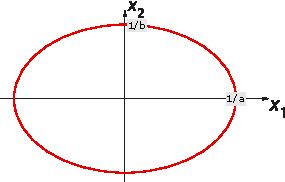
\includegraphics[width=0.45\columnwidth]{10_Quadratische_Formen/ellipse.pdf}
\end{center}
\vspace{-2mm}

\textbf{Hyperbel}\par\vskip2pt
$q(x) = a^2x_1^2 - b^2x_2^2 = 1$

\vspace{-2mm}
\begin{center}
\begin{minipage}{0.4\columnwidth}
	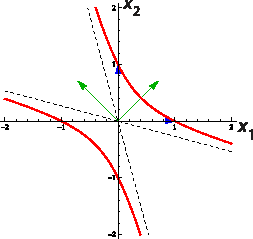
\includegraphics[width=\textwidth]{10_Quadratische_Formen/hyperbel.pdf}
\end{minipage}
\hspace{1em}%\hfill
\begin{minipage}{0.3\columnwidth}
	\textcolor{blue}{Standardbasis}\par
	\textcolor{OliveGreen}{Hauptachsenbasis}\par
	\textcolor{red}{Hyperbel}\par
	Asymptoten: $\pm\frac{a}{b}$
\end{minipage}
\end{center}
\vspace{-2mm}

\textbf{Weitere Formen}\par\vskip2pt
\begin{tabular}{ll}
	$a^2x_1^2 + b^2x_2^2 + 1 = 0$ & leere Menge \\
	$x_1^2 + b^2x_2^2 = 0$        & Punkt \\
	$x_1^2 - b^2x_2^2 = 0$        & sich schneidendes Geradenpaar \\
\end{tabular}

}
\WhiteSpace
	
\section{11. Kleinste Quadrate}
\WhiteSpace
	\subsection{11.1 Kleinste Quadrate}{
\vskip1pt

Mit dem Prinzip der \glqq kleinsten Quadrate\grqq \hskip1pt kann man zwar überbestimmte Gleichungssysteme nicht lösen, man kann jedoch eine möglichst \glqq gute\grqq \hskip1pt Lösung finden, indem man den quadratischen Fehler minimiert. \vskip5pt

\begin{minipage}{\columnwidth}
Bsp:\par
$\begin{matrix} 2x_1 & + & 3x_2 & = & 6 \\ 3x_1 & + & 4x_2 & = & 8 \\ 2x_1 & + & 1x_2 & = & 3 \end{matrix} \hskip7pt \Rightarrow$ \hskip4pt überbestimmt \vskip5pt
Wir bilden die Differenz (= Fehler) aus der rechten und der linken Seite und nennen sie Residuenvektor $r$: \vskip5pt
$\begin{matrix} 2x_1 & + & 3x_2 & - & 6 & = & r_1 \\ 3x_1 & + & 4x_2 & - & 8 & = & r_2 \\ 2x_1 & + & 1x_2 & - & 3 & = & r_3 \end{matrix}$ \vskip5pt
Wir suchen $(x_1 \hskip2pt x_2)^T$, sodass $\|r \|_2 = \|Ax-c\|_2$ minimal wird.\par%
$\Rightarrow$ quadratischer Fehler minimal
\end{minipage}

\vskip6pt

\textbf{Vorgehen:} \vskip1pt
Dazu lösen wir das Gleichungssystem $A^TAx = A^Tc$ welches in den meisten Aufgabe bereits in der Form $Ax - c = r$ gegeben ist (siehe oben).

\begin{enumerate}[label=\protect\circled{\arabic*}]
\item Man bestimme $A$ und $c$\vskip2pt
\vskip2pt Bsp: \scalebox{0.8}{\hskip8pt$A = \begin{pmatrix}2 & 3 \\ 3 & 4 \\ 2 & 1 \end{pmatrix}, \hskip5pt c = \begin{pmatrix} 6 \\ 8 \\ 3 \end{pmatrix}$} \par

\item Man berechne $A^TA$ und $A^Tc$
\vskip2pt Bsp: \scalebox{0.8}{\hskip8pt$A^TA = \begin{pmatrix}17 & 20 \\ 20 & 2 \end{pmatrix}, \hskip5pt A^Tc = \begin{pmatrix} 42 \\ 53 \end{pmatrix}$} \par

\item Man löse das Gleichungssystem $A^TAx = A^Tc$
\vskip2pt Bsp: \scalebox{0.8}{$\begin{pmatrix}17 & 20 \\ 20 & 2 \end{pmatrix}\cdot \begin{pmatrix} x_1 \\ x_2 \end{pmatrix} = \begin{pmatrix} 42 \\ 53 \end{pmatrix} \hskip3pt \Rightarrow \hskip3pt x = \begin{pmatrix} 2.67 \\ -0.17 \end{pmatrix}$} \par
\end{enumerate}

}
\WhiteSpace
	\subsection{11.2 QR-Zerlegung}{
\vskip1pt

Mit der QR-Zerlegung kann eine beliebige Matrix $A \in \mathbb{R}^{m \times n}$ in das Produkt einer orthogonalen Matrix $Q \in \mathbb{R}^{n \times n}$ und einer oberen Rechtsdreiecksmatrix $R \in \mathbb{R}^{m \times n}$ verwandelt werden:\vskip10pt

\begin{center} \fbox{$A = Q \cdot R$} \end{center}

\textbf{Vorgehen:} \vskip1pt
Wir wollen nacheinander alle Elemente unterhalb der Hauptdiagonalen von $A$ eliminieren.

\begin{enumerate}[label=\protect\circled{\arabic*}]
\item Man wähle zu eliminierendes Element und benenne es $a_{ij}$.
\vskip2pt Bsp: \scalebox{0.8}{\hskip8pt$A = \begin{pmatrix} 1 & 0 \\ 0 & 1 \\ \textcolor{Maroon}{1} & 1 \end{pmatrix} \Longrightarrow \textcolor{Maroon}{a_{31}}$ soll eliminiert werden} \par

\item Lese $i, j$ ab und notiere $a_{jj}, a_{ij}$
\vskip2pt Bsp: \scalebox{0.8}{$i = 3, j = 1 \Longrightarrow a_{jj} = 1, a_{ij} = 1$} \vskip3pt

\item Berechne $w = \sqrt{a_{jj}^2 + a_{ij}^2}$
\vskip2pt Bsp: \scalebox{0.8}{$w = \sqrt{1^2 + 1^2} = \sqrt{2}$} \vskip3pt

\item Man finde die richtige Rotationsmatrix $Q'^T$. Man nehme zuerst die Identitätsmatrix $I \in \mathbb{R}^{m\times m}$ und setze $i_{ii} = \cos(\alpha)$, $i_{i j} = -\sin(\alpha)$, $i_{j i} = \sin(\alpha)$, $i_{jj} = \cos(\alpha)$. \par 
\vskip2pt Bsp: \scalebox{0.8}{$I = \begin{pmatrix}1 & 0 & 0 \\ 0 & 1 & 0  \\ 0 & 0 & 1\end{pmatrix} \Rightarrow Q'^T = \begin{pmatrix}\cos(\alpha) & 0 & \sin(\alpha) \\ 0 & 1 & 0  \\ -\sin(\alpha) & 0 & \cos(\alpha)\end{pmatrix}$} \vskip3pt

\item Setze in Rotationsmatrix $\sin(\alpha) = \frac{a_{ij}}{w}$ und $\cos(\alpha) = \frac{a_{jj}}{w}$ \par
\vskip2pt Bsp: \scalebox{0.8}{$Q'^T = \begin{pmatrix}1/\sqrt{2} & 0 & 1/\sqrt{2} \\ 0 & 1 &  0 \\ -1/\sqrt{2} & 0 & 1/\sqrt{2}\end{pmatrix}$} \vskip3pt

\item Berechne $Q'^T\cdot A = A'$\par
\vskip2pt Bsp: \scalebox{0.8}{$\begin{pmatrix}1/\sqrt{2} & 0 & 1/\sqrt{2} \\ 0 & 1 &  0 \\ -1/\sqrt{2} & 0 & 1/\sqrt{2}\end{pmatrix}\cdot \begin{pmatrix} 1 & 0 \\ 0 & 1 \\ 1 & 1 \end{pmatrix} = \begin{pmatrix} \sqrt{2} & 1/\sqrt{2} \\ 0 & 1 \\ 0 & 1/\sqrt{2} \end{pmatrix} $} \vskip3pt

\item Falls $A'$ keine obere Dreiecksmatrix, wiederhole (finde $Q''^T$ etc.) bis alle nötigen Elemente eliminiert.\par
\vskip2pt Bsp: \scalebox{0.8}{$Q''^T = \begin{pmatrix}1 & 0 & 0 \\ 0 & \sqrt{2}/\sqrt{3} &  1/\sqrt{3} \\ 0& -1/\sqrt{3} & \sqrt{2}/\sqrt{3}\end{pmatrix}, A'' = \begin{pmatrix} \sqrt{2} & 1/\sqrt{2} \\ 0 & \sqrt{3}/\sqrt{2} \\ 0 & 0 \end{pmatrix}$} \vskip3pt

\item Wenn $A'' = R$ gefunden, berechne $Q = (Q''^T\cdot Q'^T)^T$ \par $\Longrightarrow A = Q\cdot R$

\end{enumerate}
\vskip5pt
\textbf{Kleinste Quadrate mit QR-Zerlegung} \par
Löst man ein Optimierungsproblem mit dem Computer, liefert das in 10.1 beschriebene Verfahren ungenaue Lösungen (da numerisch instabil). Das Lösungsverfahren mittels QR-Zerlegung ist besser. \textbf{In Aufgabe nur machen, wenn explizit verlangt!} \vskip5pt

\textbf{Vorgehen:}\vskip3pt

\begin{enumerate}[label=\protect\circled{\arabic*}]
\item Man bestimme $A$ und $c$ wie bei 10.1.
\vskip2pt Bsp: \scalebox{0.8}{\hskip8pt$A = \begin{pmatrix} 1 & 0 \\ 0 & 1 \\ 1 & 1 \end{pmatrix}, \hskip5pt c = \begin{pmatrix} 1 \\  0 \\ 1 \end{pmatrix}$} \par

\item Man führe die QR-Zerlegung durch $A = Q R$
\vskip2pt Bsp: \scalebox{0.8}{$Q = \begin{pmatrix}1/\sqrt{2} & 1/\sqrt{6} & 1/\sqrt{3} \\ 0 & \sqrt{2}/\sqrt{3} &  -1/\sqrt{3} \\ -1/\sqrt{2} & 1/\sqrt{6} & 1/\sqrt{3}\end{pmatrix}, R = \begin{pmatrix} \sqrt{2} & 1/\sqrt{2} \\ 0 & \sqrt{3}/\sqrt{2} \\ 0 & 0 \end{pmatrix}  $} \vskip3pt

\item Man berechne $d = Q^T\cdot c$
\vskip2pt Bsp: \scalebox{0.8}{$d = Q^T\cdot c = \begin{pmatrix} 0 \\  \sqrt{2}/\sqrt{3} \\ 2/\sqrt{3} \end{pmatrix}$} \vskip3pt

\item Man berechne löse das Gleichungssystem $R_0\cdot x = d_0$, wobei $R_0$ die extrahierte Dreiecksmatrix aus $R$ ist und $d_0$ die dazugehörigen oberen Einträge von $d$
\vskip2pt Bsp: \scalebox{0.8}{$R_0 = \begin{pmatrix} \sqrt{2} & 1/\sqrt{2} \\ 0 & \sqrt{3}/\sqrt{2} \end{pmatrix}, \hskip3pt d_0 = \begin{pmatrix} 0 \\  \sqrt{2}/\sqrt{3} \end{pmatrix}$} \vskip3pt

\end{enumerate}

}
%\WhiteSpace

\section{12. Lineare Diff'gleichungssysteme}
\WhiteSpace
	\subsection{12.1 Lösen von homogenem Diff'gleichungssystem}{
\vskip1pt

Man sucht eine Lösung für ein System von Differentialgleichungen, gegeben in folgender Form: \vskip5pt

\begin{center}
$\begin{pmatrix} y_1'(t) \\ y_2'(t) \\ y_3'(t) \end{pmatrix} = \begin{pmatrix}a_{11} & a_{12} & a_{13}\\ a_{21} & a_{22}  & a_{23}\\ a_{31} & a_{32} & a_{33} \end{pmatrix} \cdot \begin{pmatrix} y_1(t) \\ y_2(t) \\ y_3(t) \end{pmatrix}, \hskip5pt \begin{pmatrix} y_1(0) \\ y_2(0) \\ y_3(0) \end{pmatrix}$
\end{center}

Die Anfangsbedingungen $y(0)$ sowie die Matrix A sei bekannt, gesucht ist $y(t)$. \par
Das Problem kann durch Transformation in Eigenbasis (Entkopplung) gelöst werden. \par
\vskip6pt

\begin{minipage}[t]{0.15 \columnwidth}
Bsp:
\end{minipage}
\begin{minipage}[t]{0.84 \columnwidth}
$\begin{pmatrix} y_1'(t) \\ y_2'(t) \end{pmatrix} = \begin{pmatrix}3 & 2 \\ 1 & 4 \end{pmatrix} \cdot \begin{pmatrix} y_1(t) \\ y_2(t)\end{pmatrix}, \hskip5pt \begin{pmatrix} y_1(0) \\ y_2(0) \end{pmatrix} = \begin{pmatrix} 3 \\ 6 \end{pmatrix}$
\end{minipage}

\vskip6pt

\textbf{Vorgehen:} (Transformation in Eigenbasis $z = T^{-1}\cdot y$) \vskip1pt

\begin{enumerate}[label=\protect\circled{\arabic*}]
\item Man diagonalisiere die Matrix $A = TDT^{-1}$ (siehe 6.6) und bestimme die Transformationsmatrix $T$.
\vskip2pt Bsp: \scalebox{0.8}{\hskip8pt$D = \begin{pmatrix}2 & 0 \\ 0 & 5 \end{pmatrix}, \hskip3pt T = \begin{pmatrix}-2 & 1 \\ 1 & 1 \end{pmatrix}$} \par

\item Sei $t^{(i)}$ die i-te Spalte von $T$ und $d_{ii}$ der i-te Diagonaleintrag von $D$. \par Die Lösung des Diff'gleichungssystems lautet dann:\par $y(t) = z_1(0)\cdot t^{(1)}\cdot e^{d_{11} t} + z_2(0)\cdot t^{(2)}\cdot e^{d_{22} t} + \hdots$
\vskip2pt Bsp: \scalebox{0.8}{\hskip8pt $\begin{pmatrix} y_1(t) \\ y_2(t) \end{pmatrix} = z_1(0)\cdot \begin{pmatrix} -2 \\ 1 \end{pmatrix} \cdot e^{2t} + z_2(0)\cdot \begin{pmatrix} 1 \\ 1 \end{pmatrix} \cdot e^{5t}$} \par

\item Variante 1: Bestimme $T^{-1}$, danach $z(0) = T^{-1}\cdot y(0)$. \par
Variante 2: Bestimme $z(0)$ durch Lösen des Gleichungssystems $T\cdot z(0) = y(0)$. \par
Falls keine Anfangsbedingungen gegeben, $z_i(0) = C_i$.
\vskip2pt Bsp: \scalebox{0.8}{\hskip8pt$\begin{pmatrix}-1/3 & 1/3 \\ 1/3 & 2/3 \end{pmatrix} \cdot \begin{pmatrix} 3 \\ 6 \end{pmatrix} = \begin{pmatrix} 1 \\ 5 \end{pmatrix} = \begin{pmatrix} z_1(0) \\ z_2(0) \end{pmatrix}$} \par

\end{enumerate}
\vspace{-2pt}

}
\WhiteSpace
	\subsection{12.2 Umwandlung höhere Ordnung in System 1. Ordnung}{
\vskip1pt

Man will eine Differentialgleichung höherer Ordnung in ein Differentialgleichungssystem 1. Ordnung umwandeln: \vskip5pt

\begin{minipage}[t]{0.2 \columnwidth}
Bsp:
\end{minipage}
\begin{minipage}[t]{0.79 \columnwidth}
$y'''(t) + 4\cdot y''(t) + 2\cdot y'(t) - 3 y(t) = 0$\vskip5pt $y(0) = 1, \hskip3pt y'(0) = 3, \hskip3pt y''(0 ) = 2$
\end{minipage}




\vskip6pt

\textbf{Vorgehen:} \vskip1pt

\begin{enumerate}[label=\protect\circled{\arabic*}]
\item Man substituiere $y = y_0, y' = y_1$ etc. Die höchste Ableitung lasse man stehen.
\vskip2pt Bsp: \scalebox{0.8}{\hskip8pt $y'''(t) + 4\cdot y_2(t) + 2\cdot y_1(t) - 3 y_0(t) = 0$} \par

\item Man ersetze höchste Ableitung durch einfache Ableitung mit Substitution.
\vskip2pt Bsp: \scalebox{0.8}{\hskip8pt $y_2'(t) + 4\cdot y_2(t) + 2\cdot y_1(t) - 3 y_0(t) = 0$} \par

\item Durch die Substitution hat man automatisch ein Diff'gleichungssystem erster Ordnung erzeugt: \par
\vskip2pt Bsp: \scalebox{0.8}{\hskip8pt$\begin{matrix} y_0' & =  & y_1 \\ y_1' & = & y_2 \\ y_2' & =  & 3\cdot y_0 & -  &2\cdot y_1 & -& 4 \cdot y_2\end{matrix}$} \par

\item Zum Schluss substituiere noch die Anfangsbedingungen \par
\vskip2pt Bsp: \scalebox{0.8}{\hskip8pt$y_0(0) = 1, \hskip3pt y_1(0) = 3, \hskip3pt y_2(0) = 2$} \par

\end{enumerate}

}
	\subsection{12.3 Lösen von inhomogenem Diff'gleichungssystem}{
\vskip1pt

Man hat bereits mit dem in 11.1 beschriebenen Verfahren die Lösung $y_h(t)$ für das homogene Diff'gleichungssystem $y' = A\cdot y$ gefunden. Jetzt sucht man die Lösung für das inhomogene System: \vskip5pt
\begin{center}
$y' = A\cdot y + b$: \vskip5pt
\end{center}
\vskip5pt
Das Prinzip ist, dass man eine partikuläre Lösung $y_p(t)$ findet, die die Diff'gleichung sicher erfüllt. Die allgemeine Lösung ist dann $y(t) = y_h(t) + y_p(t)$ \par
\vskip6pt

\textbf{Vorgehen:} \vskip1pt

\begin{enumerate}[label=\protect\circled{\arabic*}]
\item Man nimmt an, dass die partikuläre Lösung $y_p(t)$ konstant ist. Daraus folgt, dass $y_p'(t) = 0$. Man löse also das Gleichungssystem $A \cdot y_p = -b$

\item Man addiere die homogene und die Partikuläre Lösung zusammen: $y(t) = y_h(t) + y_p(t)$

\end{enumerate}

}
\WhiteSpace
	\subsection{12.4 Bedingungen im Unendlichen}{
\vskip1pt

Für das Bestimmen der Konstanten $C_i$ sind nicht immer nur Anfangsbedingungen $y_i(0)$ gegeben, sondern manchmal auch Bedingungen wie $\lim\limits_{t \rightarrow \infty}{y_i(t)} = a$. \vskip6pt

Bsp: \hskip6pt Bestimme $C_i$ von $y(t) = C_1 + 3C_2e^{-t} + C_3\cdot e^{2t}$ \vskip2pt
\hskip22pt mit $y(0) = 2$ und $\lim\limits_{t \rightarrow \infty}{y(t)} = 5$

\vskip5pt

\textbf{Vorgehen:} \vskip1pt

\begin{enumerate}[label=\protect\circled{\arabic*}]
\item Verlangt eine Bedingung, dass $y(t)$ im Unendlichen beschränkt sein soll, setze Konstanten vor Exponentialfunktionen mit positiven Exponenten null.
\vskip2pt Bsp: \scalebox{0.9}{\hskip8pt Zweite Bedingung $\lim\limits_{t \rightarrow \infty}{y(t)} = 5 \hskip3pt \Rightarrow \hskip3pt C_3 = 0$} \par

\item Man bestimme weitere Konstanten, indem man $t \rightarrow \infty$ einsetzt.
\vskip2pt Bsp: \scalebox{0.9}{\hskip8pt$\lim\limits_{t \rightarrow \infty}{y(t)} = C_1 = 5$} \par

\item Man bestimme die übrigen Konstanten, indem man $t = 0$ einsetzt.
\vskip2pt Bsp: \scalebox{0.9}{\hskip8pt $ y(0) = 5 + 3 C_2 = 2 \hskip3pt \Rightarrow \hskip3pt C_2 = -1$} \par
\end{enumerate}

}
\WhiteSpace
	
\section{13. Weiteres}
\WhiteSpace
	\subsection{13.1 Winkeltabelle}{
\vskip1pt

\begin{tabularx}{0.99\columnwidth}{X|YYYYYYYYY}
%\begin{tabular*}{\columnwidth}{@{\extracolsep{\fill}}l|ccccccccc}
	rad     & 0 &   $\frac{\pi}{6}$    &   $\frac{\pi}{4}$    &   $\frac{\pi}{3}$    &   $\frac{\pi}{2}$    &   $\frac{2\pi}{3}$   &   $\frac{3\pi}{4}$   &   $\frac{5\pi}{6}$    & $\pi$ \\
	$\circ$ & 0 &          30          &          45          &          60          &          90          &          120         &         135          &          150          &  180  \\ \hline
	sin     & 0 &     $\frac{1}{2}$    & $\frac{\sqrt{2}}{2}$ & $\frac{\sqrt{3}}{2}$ &         $1$          & $\frac{\sqrt{3}}{2}$ & $\frac{\sqrt{2}}{2}$ &     $\frac{1}{2}$     &  $0$  \\
	cos     & 1 & $\frac{\sqrt{3}}{2}$ & $\frac{\sqrt{2}}{2}$ &     $\frac{1}{2}$    &         $0$          &    $-\frac{1}{2}$    &$-\frac{\sqrt{2}}{2}$ &$-\frac{\sqrt{3}}{2}$  &  $-1$ \\
	tan     & 0 & $\frac{1}{\sqrt{3}}$ &         $1$          &      $\sqrt{3}$      &         $-$          &      $-\sqrt{3}$     &         $-1$         & $-\frac{1}{\sqrt{3}}$ &  $0$  \\
\end{tabularx}

}
\WhiteSpace
	\subsection{13.2 Givens-Rotation}{
\vskip1pt

Die Givens-Rotation ermöglicht eine Rotation um eine fixe Achse in $\mathbb{R}^3$ mit Orthonormalbasis.\par

\begin{center}
$U_x(\phi) := \begin{pmatrix}
				      1       &       0       &      0       \\
			          0       &  \cos(\alpha) & -\sin(\alpha)\\
				      0       & \sin(\alpha)  &  \cos(\alpha) 
			  \end{pmatrix}$\vskip3pt\par
$U_y(\phi) := \begin{pmatrix}
			     \cos(\alpha) &       0       &  \sin(\alpha) \\
				       0      &       1       &      0        \\
				-\sin(\alpha) &       0       &  \cos(\alpha)
			  \end{pmatrix}$\vskip3pt\par
$U_z(\phi) := \begin{pmatrix}
			     \cos(\alpha) & -\sin(\alpha) &      0       \\
				 \sin(\alpha) &  \cos(\alpha) &      0       \\
				      0       &       0       &      1
			  \end{pmatrix}$\par	  
\end{center}

\textbf{Charakteristisches Polynom}\par\vskip1pt
Sie besitzt das charakteristische Polynom
\begin{center}
$(1 - \lambda)(\lambda^2 -2\lambda cos(\alpha) + 1) = 0$
\end{center}
\vskip3pt

\textbf{Eigenwerte}\par\vskip2pt
Und die Eignewerte ergeben sich wie folgt

\vspace{-7pt}
\begin{align*}
\lambda_1 &= 1 \\
\lambda_2 &= cos(\alpha) + isin(\alpha) \\
\lambda_3 &= cos(\alpha) - isin(\alpha)
\end{align*}
\vspace{-7pt}

Dabei ergeben sich die Eigenvektoren zu
\begin{center}
$v_1 = \begin{pmatrix} 1\\ 0\\ 0\end{pmatrix}, \qquad v_2 = \begin{pmatrix} 0\\ i\\ 0\end{pmatrix}, \qquad v_3 = \begin{pmatrix} 0\\ -i\\ 0\end{pmatrix}$
\end{center}

}
\WhiteSpace
	\subsection{13.3 Blockmatrix}{
\vskip1pt

Eine Blockmatrix ist eine Matrix welche in mehrere \grqq{}Blöcke\grqq{} unterteilt werden kann.\par

Beispiel einer $2 \times 2$ Blockmatrix:
\begin{center}
$P = \begin{bmatrix}
			\pmb A & \pmb B \\
			\pmb C & \pmb D
	 \end{bmatrix}$
\end{center}

\textbf{Determinante}\par\vskip1pt
Für die Determinante einer $2 \times 2$ Blockmatrix mit einem 0 Block gilt die Eigenschaft\par\vspace{-4pt}
\begin{center}
$det\begin{pmatrix} \pmb A & 0\\	\pmb C & \pmb D\end{pmatrix} = det(\pmb A)det(\pmb B)$
\end{center}\par\vskip3pt

Handelt es sich bei den Blöcken um quadratische Matrizen der gleichen Größe, welche kommutieren ($CD = DC$) dann gilt des Weiteren\par\vspace{-4pt}
\begin{center}
$det\begin{pmatrix} \pmb A & \pmb B\\ \pmb C & \pmb D\end{pmatrix} = det(\pmb{AD} - \pmb{BC})$
\end{center}\par\vskip3pt

Und falls $A=D$ und $B=C$ gilt\par\vspace{-4pt}
\begin{center}
$det\begin{pmatrix} \pmb A & \pmb B\\ \pmb B & \pmb A\end{pmatrix} = det(\pmb A - \pmb B)det(\pmb A + \pmb B)$
\end{center}\par\vskip3pt


\textbf{Eigenwerte}\par\vskip1pt
Die Eigenwerte einer $2 \times 2$ Blockmatrix $P$ mit einem 0 Block ergeben sich aus\par\vspace{-4pt}
\begin{center}
$det\begin{pmatrix} \pmb A - \lambda\pmb I & 0\\ \pmb C & \pmb D - \lambda\pmb I\end{pmatrix} = det(\pmb A - \lambda\pmb I)det(\pmb D - \lambda\pmb I)$
\end{center}\par\vskip3pt

Deshalb gilt $eig(P) = (eig(A), eig(D))$

}
\WhiteSpace
	\subsection{13.4 Matrixexponentialfunktion}{
\vskip1pt

Die Matrixexponentialfunktion wird auf quadratischen Matrizen angewendet und ist definiert wie folgt\par

\vspace{-12pt}
\begin{center}
\[e^{A} = \sum_{n=0}^\infty\frac{A^n}{n!}= I + A + \frac{A^2}{2} + ...\]
\end{center}

\textbf{Aehnlichkeitstransformation} \par\vspace{-3pt}
\[e^A = e^{TDT^{-1}} = T\cdot diag(e^{\lambda_1}, \hdots, e^{\lambda_n})\cdot T^{-1}\]

}
\WhiteSpace
	\subsection{13.5 Spur}{
\vskip1pt

Die Spur einer quadratischen $n \times n$ Matrix $A$ bezeichnet die Summe ihrer Hauptdiagonalelemente.\par\vskip2pt

\begin{center}
$A=\begin{pmatrix}
	a_{11} & a_{12} & \cdots & a_{1n} \\
	a_{21} & a_{22} & \cdots & a_{2n} \\
	\vdots & \vdots & \ddots & \vdots \\
	a_{n1} & a_{n2} & \cdots & a_{nn}
	\end{pmatrix}$
\end{center}
\vspace{-5pt}

ist also\par\vspace{-15pt}
\begin{center}
\[Spur(A)=\sum_{j=1}^n a_{jj} = a_{11}+a_{22}+\dotsb+a_{nn}\]
\end{center}
\vspace{-5pt}

\textbf{Eigenschaften:}
\vspace{-3pt}

\begin{itemize}[leftmargin=0.29cm, itemsep=0.5pt]
\item $Spur(A) = Spur(A^T)$.
\item $Spur(\alpha A + \beta B) = \alpha Spur(A) + \beta Spur(B)$.
\item $Spur(AB) = Spur(BA)$ beides mit $\textstyle\sum_{i,j}a_{ij}b_{ji}$
\item $Spur(ABC) = Spur(CBA) = Spur(BCA)$
\item $Spur(B^{-1}AB) = Spur(A)$
\item Sind $A$ und $B$ $n\times n$ Matrizen, wobei $A$ positiv definit und $B$ nicht negativ ist, so gilt $Spur(AB) \geq 0$.
\end{itemize}

}
\colbreak
%\WhiteSpace
	
\section{14. Persönliche Ergänzungen}
\WhiteSpace
\colbreak
\mbox{}
	
\end{multicols*} 

\end{document}